%!TEX root = ../thesis.tex
%*******************************************************************************
%****************************** Third Chapter **********************************
%*******************************************************************************
\chapter{Selecting Heavy Neutral Leptons}
\label{ChapterSelect}

% **************************** Define Graphics Path **************************
\ifpdf
    \graphicspath{{Chapter9/Figs/Raster/}{Chapter9/Figs/PDF/}{Chapter9/Figs/}}
\else
    \graphicspath{{Chapter9/Figs/Vector/}{Chapter9/Figs/}}
\fi

%********************************** %Opening  **************************************

The search of HNLs begins with a selection performed on Monte Carlo (MC) samples, which was simulated using the simulation detailed in Chapter \ref{ChapterSim} and then reconstructed using the framework detailed in Chapter \ref{ChapterReco}.
This is the very first exploration of SBND physics capabilities in the HNL regime, and this selection provides the first benchmark for understanding the current reconstruction performance of HNL signals based on MC.
The selection first exploits the boosted kinematic features of HNL showers using the reconstructed calorimetry from the TPC and PDS combined.                                                                                 
Then, the reconstructed timing resolution is the parameter of interest since the selection relies on the late arrival of HNLs compared to SM neutrinos.
Ideally, this selection procedure can be carried out on real data once the detector is operational.

The following chapter will provide details on the selection workflow to identify HNL signals from backgrounds.
The definition of the signal and background topology is first discussed in Sec. \ref{sec:sig_bkg_def}.
This is followed by Sec. \ref{sec:select_mc} describing the MC samples.
Sec. \ref{sec:key_dist} describes the beam bucket distribution, which is the key distribution used for evaluating the selection.
The first stage of the selection is to reject cosmic backgrounds as discussed in Sec. \ref{sec:cosmic_rej} and 
the second stage is to reject SM neutrino backgrounds as discussed in Sec. \ref{sec:sm_rej}.                   
Then, Sec. \ref{sec:hnl_shower_select} details the last stage of the selection to identify HNL showers from trickier shower-like backgrounds.
The result of the selection procedure is summarised in Sec. \ref{sec:select_result}.                           
Furthermore, a hypothetical question is proposed in Sec. \ref{sec:truth_bucket}, driven by the timing resolution observed in reconstruction, if better sensitivity limits can be achieved given an improvement in timing resolution. 
Finally, a concluding remark is provided Sec. \ref{sec:select_conclude}.

\clearpage
%********************************** %First Section  **************************************

\section{Signal and Background Definition}
\label{sec:sig_bkg_def}

A selection begins with defining the signal topology to be selected, namely $\pi^0 \rightarrow \gamma\gamma$ showers resulting from HNLs decaying inside the Fiducial Volume (FV) of the SBND detector.
FV is defined as a smaller volume approximately 70\% of the active volume, to be defined in the forthcoming Sec. \ref{sec:fv_cut}.
The di-photon showers of HNLs result in one or more showers without any hadronic activities at the vertex.
Fig. \ref{fig:hnl_evd_1shw} shows an event display of two observable distinct photon showers.  
In the case where only a single shower is reconstructed, two scenarios can happen.
The first scenario is that only a single photon shower deposits energy inside the detector while the other one escapes.
The second scenario is that the di-photon showers are very boosted and forward-going.
Fig. \ref{fig:pi0_distribution} has previously shown that the angle of $\pi^0$ to the beam direction is very small $< 30^\circ$ for HNLs in the mass range of 140-260 MeV.
Thus, the resulting di-photon showers can overlap each other and the opening angle between the two showers is too small to be reconstructed as two distinct showers. 
Fig. \ref{fig:hnl_evd_2shw} shows an event display of very boosted di-photons showers, which is likely to be reconstructed as a single energetic shower.

\begin{figure}[htbp!]
	\centering
        \begin{subfigure}[b]{0.85\textwidth}  
            \centering 
            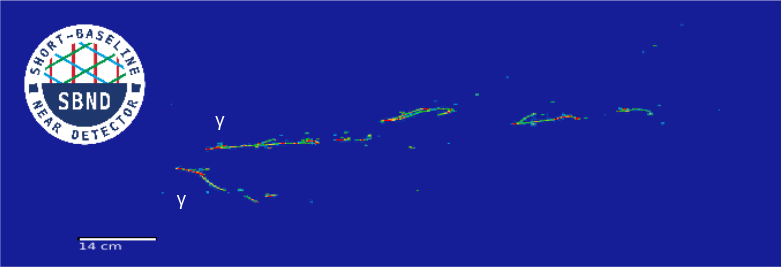
\includegraphics[width=\textwidth]{hnl_2shw}
            \caption{}%
	    \label{fig:hnl_evd_1shw}
        \end{subfigure}
        \centering
        \begin{subfigure}[b]{0.85\textwidth}   
            \centering 
            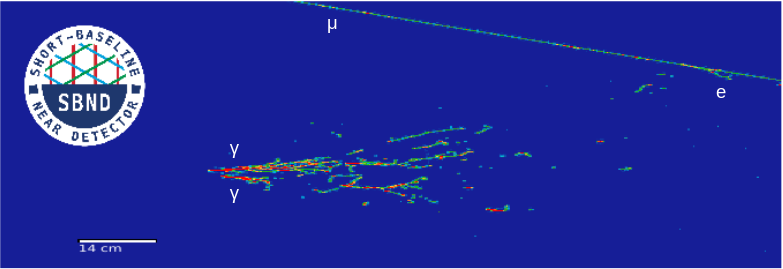
\includegraphics[width=\textwidth]{hnl_1shw}
            \caption{}%
	    \label{fig:hnl_evd_2shw}
	\end{subfigure}
        \caption{
		Event displays showing two different topologies observed from di-photon showers from HNLs. 
	}
        \label{fig:hnl_evd_select}
\end{figure}

%SM neutrino background
Given this signal topology, the first-order background topology from SM neutrino is Neutral Current interactions that produce $\pi^0$ (NC $\pi^0$).
This interaction type also produces di-photon showers without any hadronic activities at the vertex.
The second-order background topology is from Charged Current electron (anti-)neutrinos (CC $\nu_e$) interactions.
This interaction type typically produces one or multiple hadrons in addition to a single shower.
However, in some scenarios, the hadrons are too low in energy to be reconstructed, resulting in a single shower topology after reconstruction.
Fig. \ref{fig:ncpi0_evd} shows an event display of the observable di-photon showers from NC $\pi^0$ interaction, which is indistinguishable from the di-photon showers from HNLs.
The key distinction separating HNL showers from these SM neutrino showers is the boosted topology of HNL showers, which is exploited for selection to be detailed in Sec. \ref{sec:hnl_shower_select}.

\begin{figure}[htbp!]
	\centering
        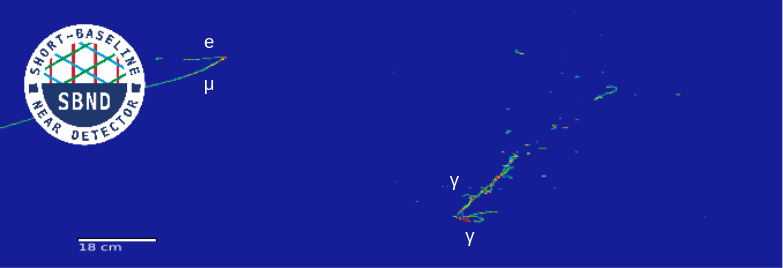
\includegraphics[width=0.85\textwidth]{ncpi0}
        \caption{
		Event display showing di-photon showers from NC $\pi^0$ interactions. 
	}
	\label{fig:ncpi0_evd}
\end{figure}

Moreover, SM neutrino interactions can occur outside the FV, but their products can have sufficient energy to propagate inside the FV.
For those interactions occurring outside the FV but inside the detector, they are considered Non-FV interactions.
Those interactions occurring completely outside of the detector are considered dirt neutrino interactions.
As previously discussed in Sec. \ref{sec:gen_genie}, despite interacting outside of the FV, these interactions can introduce non-negligible backgrounds, especially if their daughter particles produce shower final states. 

%Cosmic background and CCnumu
Finally, any background interactions that produce tracks are considered low-priority backgrounds since a track topology is easily distinguishable from a shower topology.
From SM neutrinos, these interactions are from Charged Current muon (anti-)neutrinos (CC $\nu_\mu$) or any Neutral Current interactions that do not produce a neutral pion (Other NC).
The track signature for protons is short stubs, while the track signature for muons and pions is long tracks.
Fig. \ref{fig:numu_cos_evd} shows an event display of a common observable from CC $\nu_\mu$ interactions that result in a final state of 1 muon and 1 proton.                                                   
Similarly, cosmic muons typically leave very long tracks crossing the entire detector with some iconic features such as delta-rays or Michel electrons, which are electrons from muons that decay at rest.
Fig. \ref{fig:hnl_evd_2shw} (top right) and Fig. \ref{fig:numu_cos_evd} (bottom left) both show a long cosmic track with some delta-rays along the track.
Meanwhile, Fig. \ref{fig:ncpi0_evd} shows a cosmic muon comes to a stop and eventually decays into a Michel electron (top left).

\begin{figure}[htbp!]
	\centering
        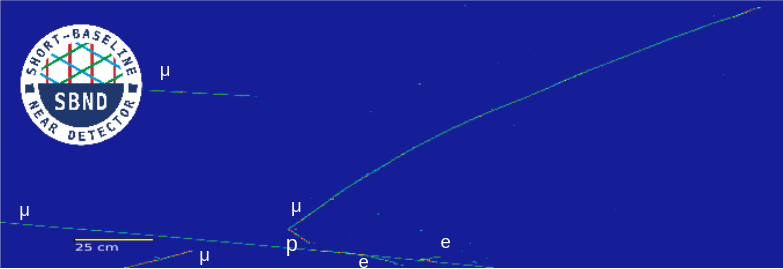
\includegraphics[width=0.85\textwidth]{1m1p_cos}
        \caption{
		Event display showing 1 muon and 1 proton track from CC $\nu_\mu$ interactions. 
	}
	\label{fig:numu_cos_evd}
\end{figure}


%********************************** %First Section  **************************************

\section{Description of MC Samples}
\label{sec:select_mc}

%The selection presented in this chapter was performed on Monte Carlo (MC) samples, that were generated using the simulation framework described in Chapter \ref{ChapterSim}.
%These samples were then reconstructed using the framework described in Chapter \ref{ChapterReco}.

For signal MC samples, HNL signals were overlaid with cosmic muons occurring within the TPC readout window.
In total, 7 samples were generated, where each sample of 60,000 signals corresponds to a mass point ranging between 140 to 260 MeV in the step of 20 MeV.
The signals can be re-weighted from the nominal mixing angle $|U_{\mu4}|^{2}$ to another mixing angle $|U'_{\mu4}|^{2}$ by applying a weight as follows
\begin{equation}
    w = \left(\frac{|U_{\mu4}|^{2}}{|U'_{\mu4}|^{2}}\right)^{2}
\end{equation}

For SM neutrino MC samples, three samples were produced.
The first one is a core sample entailing all SM neutrino interactions occurring inside the detector volume as well as outside the detector in the \textit{Rockbox} volume, as discussed in Sec. \ref{sec:gen_genie}.
Two additional dedicated samples of enriched NC $\pi^0$ and CC $\nu_e$ backgrounds were also generated, to improve the limited statistics of these interactions in the core sample.
The three samples were normalised to an exposure of $1 \times 10^{21}$ Protons On Target (POT) to account for 3 years of data taking.
This yields $\sim331,000$ NC $\pi^0$ interactions and $\sim33,000$ CC $\nu_e$ interactions which are the primary background.
Other background from CC $\nu_\mu$ and other NC interactions make a total of $\sim5$ million interactions.
An additional $\sim2$ million and $\sim3$ million interactions from Non-FV and dirt interactions are also considered as backgrounds, although only a fraction of the might deposit energy in the detector.

Finally, a cosmic-only sample was generated to account for in-time cosmics, as discussed in Sec. \ref{sec:gen_corsika}.
This sample consists of events triggered by cosmic-only interactions.
However, it is important to note that a dedicated trigger efficiency study will be carried out to better understand the rate of in-time cosmic events once SBND is operational.
The cosmic-only sample was also normalised to the target POT, and combined with SM neutrino samples to form a single sample describing the background to the HNL signal.  

The unit of the selection relies on \textit{events}, defined by the triggering of the detector where a single event corresponds to a single trigger.
After reconstruction, each event contains \textit{slices}, a reconstruction unit created by Pandora that encapsulates all energy in the TPC from a single origin describing an interaction, as discussed in Sec. \ref{sec:reco_tpc}.        
The equivalent reconstruction unit to a slice from the PDS reconstruction is a \textit{flash}, as discussed in Sec. \ref{sec:reco_others}.
A slice consists of a hierarchy of particles, where each can resemble a track or a shower.
The selection presented in the forthcoming sections is performed on slices, where slices are accepted or rejected based on the series of cuts using the reconstructed information within the slice or by matching a slice to a flash.

%********************************** %First Section  **************************************

\section{Key Distribution in HNL Search}
\label{sec:key_dist}

The selection workflow was developed by exploiting distinct features of HNLs, separating signal topologies from background topologies.
One previously stated feature is the boosted topology of HNL showers as depicted in Fig. \ref{fig:hnl_evd_1shw}.
Another feature is the late arrival of HNLs relative to SM neutrinos, as previously depicted in Fig. \ref{fig:beam_modulus} showing the timing distribution of the beam bucket for HNLs and SM neutrinos.
The distribution of SM neutrinos resembles a Gaussian-shaped bucket as they travel nearly at the speed of light, whilst HNLs travel at a slower velocity and smear the Gaussian.
This is the key distribution for setting the upper limits on the mixing angle $|U_{\mu4}|^2$ of HNLs since it demonstrates the distinct shape difference between the signal and the background, which is required by the setting limits procedure to be discussed in Chapter \ref{ChapterResult}.

To reconstruct the beam bucket distribution, the required information is the flash time matched to a slice that corresponds to the start time $t_0$ of the interaction.
The arrival time at the upstream wall of the detector is then computed from the flash time, equivalent to a shift from the interaction vertex $z$-position to $z = 0$.
The arrival time corresponds to 81 beam buckets in a single beam spill and thus, to overlay 81 buckets as a single one, a modulus of 18.936 ns is applied.
The reconstructed beam bucket for SM neutrinos resembles a Gaussian with a sigma of $2.26$ ns as compared to the proton bucket from the Booster synchrotron with an intrinsic sigma of $1.308$ ns.
Discussion on different smearing contributors to the beam bucket reconstruction will be detailed later in Sec. \ref{sec:truth_bucket}.
The beam bucket distribution will be shown repeatedly throughout the following sections to demonstrate the impacts of the selection.

%********************************** %First Section  **************************************

\section{Cosmic Background Removal}
\label{sec:cosmic_rej}

\subsection{Pandora Unambiguous Cosmic Removal}

Being a surface detector, SBND is exposed to a high rate of cosmic rays, expecting $\sim 185$ million reconstructed slices from cosmics for the target POT of $1 \times 10^{21}$.
As a comparison, the expected rate of reconstructed slices from SM neutrino interactions is $\sim 11$ million slices.
The first step of the selection is cosmic rejection, targeting primarily at removing out-of-time cosmic muons.
Pandora performs an unambiguous cosmic removal early in the reconstruction chain, by reconstructing a slice as a neutrino only if the slice is identified as a non-clear cosmic, as previously described in Sec. \ref{sec:reco_tpc}. 
The selection thus begins with selecting only slices reconstructed as a neutrino.
This rejects $90 \%$ of the $\sim 185$ million slices from cosmic, leaving behind only $19.5$ million slices.
Meanwhile, only $0.6 \%$ of the reconstructed slices from HNL signals are removed, with similar reductions across different SM neutrino interactions.  
The remaining slices after the cut are reconstructed as neutrinos and thus, consist of a reconstructed vertex and dedicated reconstruction algorithms required by the upcoming cuts.

For monitoring and quantifying the impacts of subsequent cuts, the efficiency of background and signal are computed from this cut onwards.
The efficiencies are defined as
\begin{align}
	\mathrm{Signal\ Efficiency = \frac{\#\ of\ selected\ signal\ slices\ with\ completeness\ >\ 50\ \%}{\#\ of\ signal\ slices\ reconstructed\ by\ Pandora\ as\ neutrinos}} \\
	\mathrm{Background\ Efficiency = \frac{\#\ of\ selected\ background\ slices}{\#\ of\ background\ slices\ reconstructed\ by\ Pandora\ as\ neutrinos}}
\end{align}
Additional completeness of 50 \% is required for signal slices to prevent double counting, such that only well-reconstructed signal slices are considered for the counting.                                    
The selection aims for a high background \textit{rejection} efficiency without compromising the signal \textit{selection} efficiency.                                                                             
This is equivalent to achieving a low background efficiency and a high signal efficiency.
Both of these efficiency numbers will be discussed for each cut and be included in the legends of the upcoming plots.                                                                                             


\subsection{Beam Spill Cut}

The second cut to remove cosmics is to consider the flash time of a slice, corresponding to the start time $t_0$ of an interaction. 
Only slices matched to a valid flash are selected, implying that each selected slice has a reconstructed flash time.
Moreover, the time of the matched flash is required to be within the beam spill window.
In the simulation of MC samples, the beam spill window is configured to be between [0.367, 1.967] $\mu$s, with $t = 0\ \mu$s corresponding to the first POT of a beam spill.
Moreover, an interaction can occur anywhere along the 500 m $z$-length of the detector, equivalent to a smearing of 17 ns in timing.
Thus, the beam spill acceptance window is widened to [0.350, 1.984] $\mu$s, as demonstrated in Fig. \ref{fig:beamspill_cut}.
The cut rejects $4$ million cosmic slices while minimally reduces signal efficiency by $3\%$.
Fig. \ref{fig:bb_beamspill} shows the beam bucket distribution after applying the cut, where two components of cosmic rays can be observed.
There is a flat distribution coming from out-of-time cosmics and a very small Gaussian-shaped distribution coming from in-time cosmics.

\subsection{CRUMBS Cut}

The third cut targets the out-of-time cosmic components by employing the CRUMBS score of a slice, which is a BDT trained to distinguish between a neutrino-like slice and a cosmic-like slice as discussed in Sec. \ref{sec:crumbs}.                                                                                       
The score distribution of CRUMBS is plotted in Fig. \ref{fig:crumbs_cut}, showing a good separation between neutrino-like and cosmic-like.                                                                        
A cut is placed to reject any slices with CRUMBS scores less than 0, effectively removing $14$ million of the remaining cosmic slices.
Comparison between Fig. \ref{fig:bb_beamspill} and \ref{fig:bb_crumbs}, before and after the CRUMBS cut, demonstrates that the majority of the removed comics are the out-of-time component. 
The remaining cosmic slices are the in-time component, concentrating at the centre of the beam bucket.  
This cut results in an effective background rejection as the background efficiency is reduced more than half from $8.3 \times 10^{-1}$ to $3.0 \times 10^{-1}$, whilst the signal efficiency only drops by $5 \%$ given the shower topology is very distinguishable from cosmic tracks.
By the end of the cosmic background removal stage, only $\sim432,000$ of the starting $185$ million cosmic slices remain, equivalent to a $99.9\%$ removal of the starting cosmic background.

\begin{figure}[h!]
        \centering
        \begin{subfigure}[b]{0.495\textwidth}
            \centering
            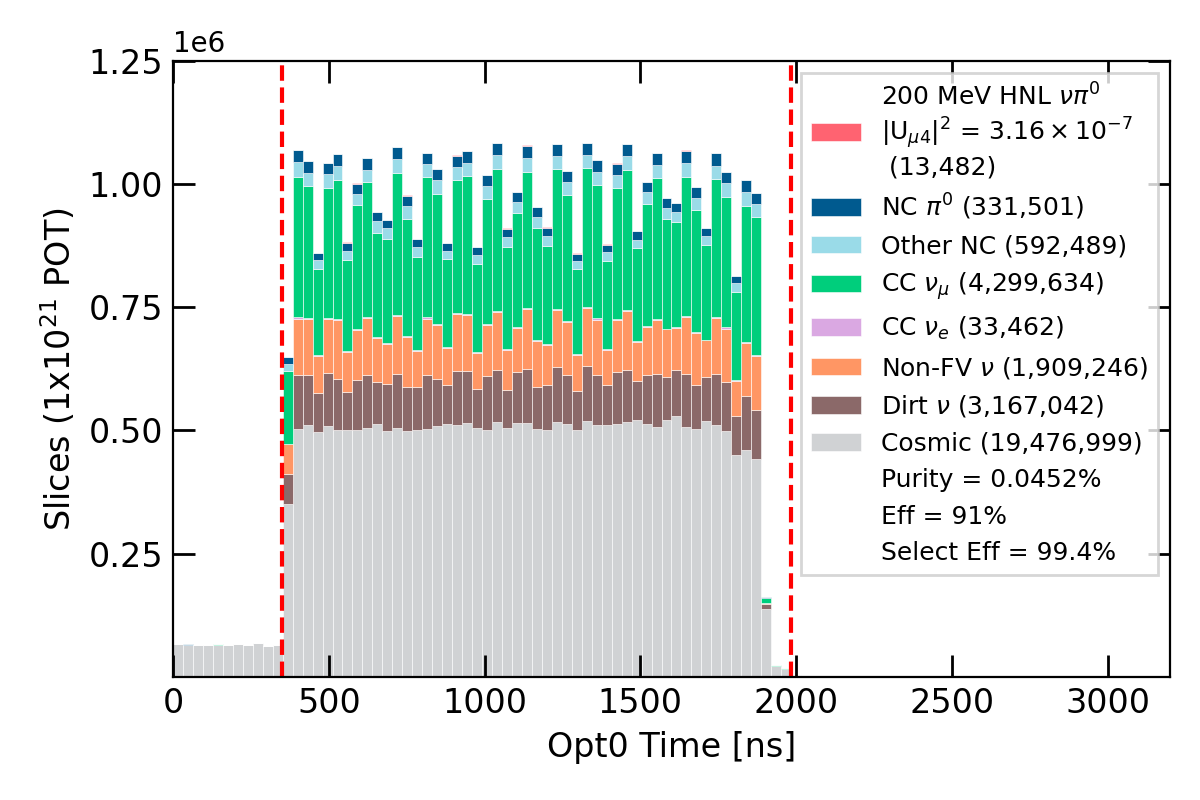
\includegraphics[width=\textwidth]{beamspill}
            \caption{Beam spill cut}%
            \label{fig:beamspill_cut}
        \end{subfigure}
        \hfill
        \begin{subfigure}[b]{0.495\textwidth}  
            \centering 
            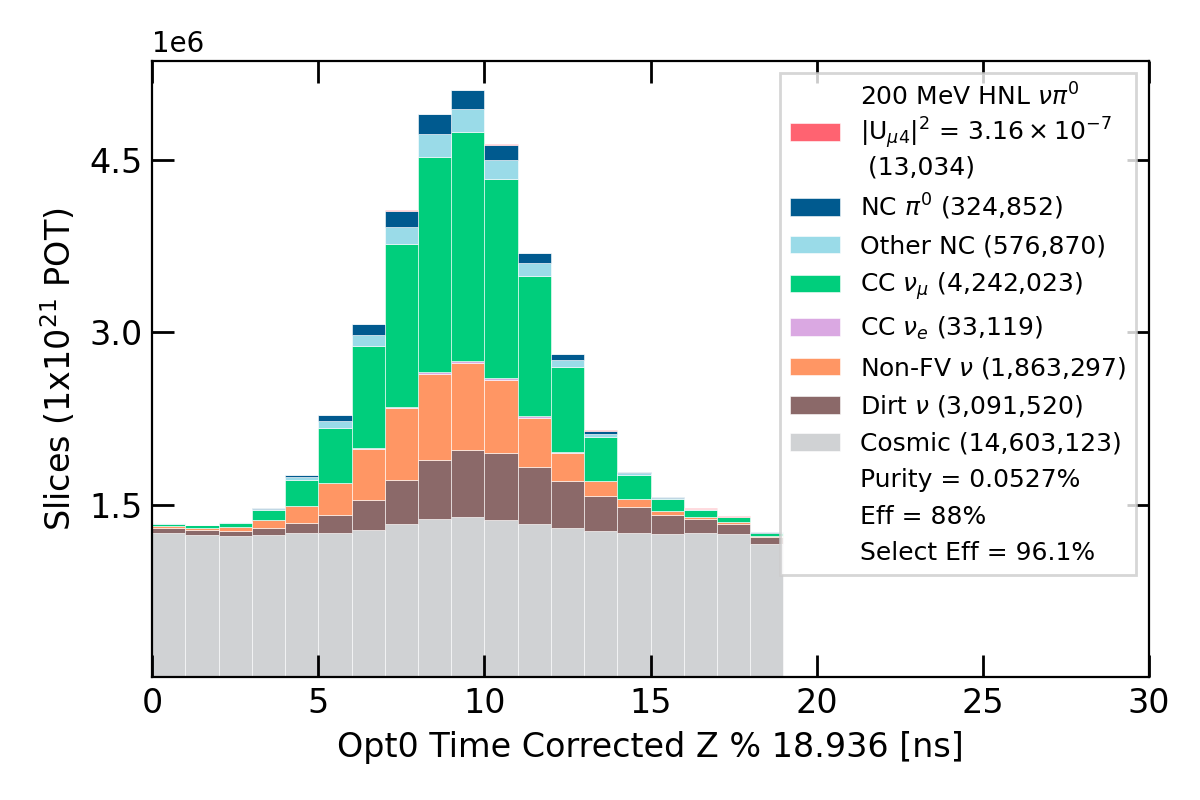
\includegraphics[width=\textwidth]{beam_bucket_post_beamspill}
            \caption{After beam spill cut}%
            \label{fig:bb_beamspill}
        \end{subfigure}
        \begin{subfigure}[b]{0.495\textwidth}   
            \centering 
            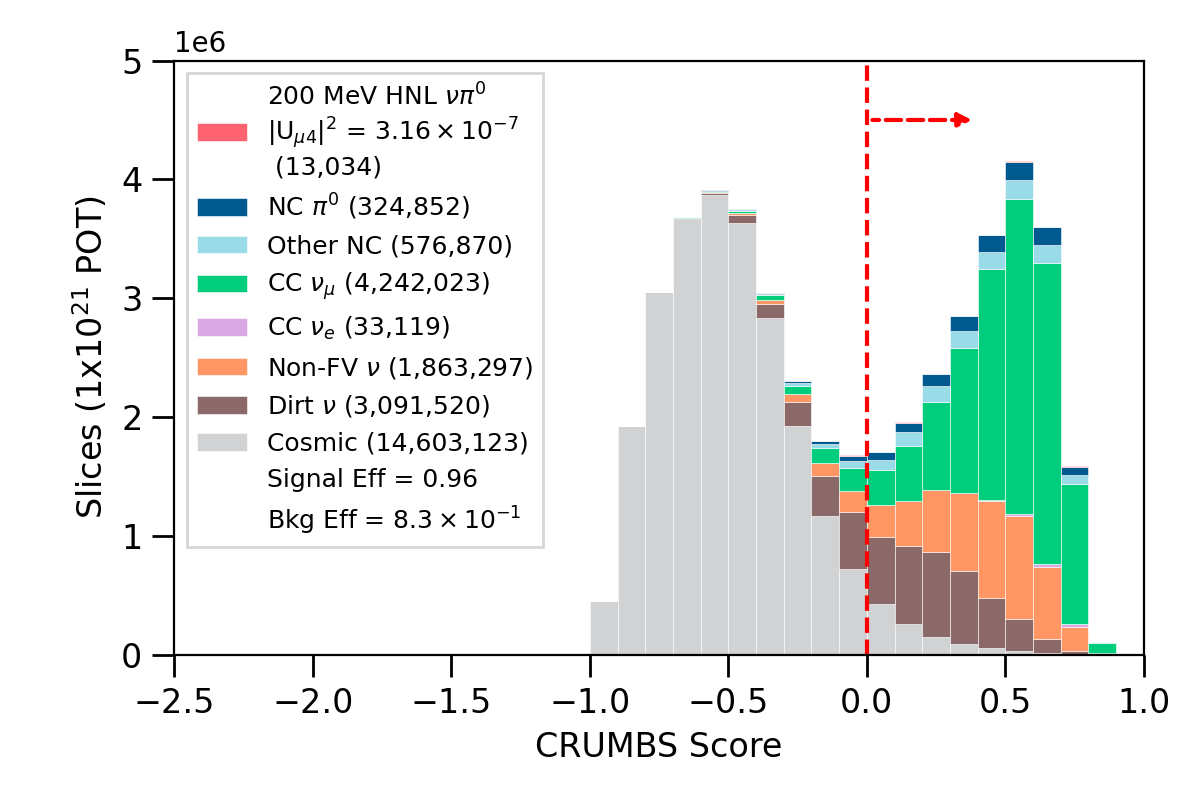
\includegraphics[width=\textwidth]{crumbs_precut}
            \caption{CRUMBS cut}%
            \label{fig:crumbs_cut}
        \end{subfigure}
        \hfill
        \begin{subfigure}[b]{0.495\textwidth}   
            \centering 
            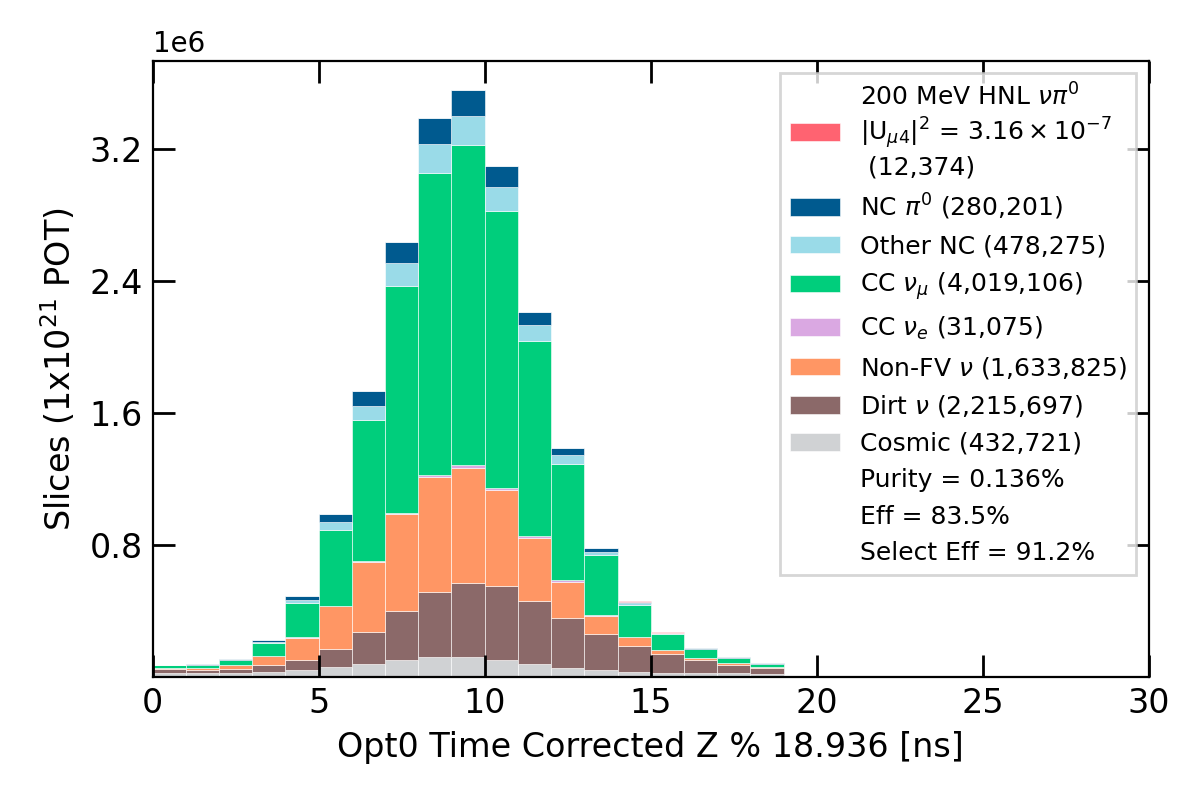
\includegraphics[width=\textwidth]{beam_bucket_post_crumbs}
            \caption{After CRUMBS cut}%
            \label{fig:bb_crumbs}
        \end{subfigure}
        \caption{
		Plots demonstrating the comic background removal cuts (left column) and the resulting beam bucket distribution after each cut (right column). 
	}
        \label{fig:cosmic_cut}
\end{figure}

\section{SM Neutrino Background Removal}
\label{sec:sm_rej}

\subsection{Fiducial Volume Cut}
\label{sec:fv_cut}

After the cosmic background removal, the next cut aims to remove backgrounds from Non-FV neutrinos and dirt neutrinos that interact outside of the FV but their products can deposit energy inside the FV. 
The cut requires the reconstructed vertex of a slice to be inside the FV of SBND, which is  defined as follows
\begin{itemize}
        \item $x$-position: $- 180 < x < -5 , 5 < x < 180$ cm
        \item $y$-position: $-180 < y < 180$ cm
        \item $z$-position: $10 < z < 450$ cm
\end{itemize}
The boundary is set on the $x$-axis to reject vertices reconstructed close to the anode and cathode.
Vertices close to the cathode might suffer from poor reconstruction due to SCE.
Meanwhile, vertices close to the anode might also indicate particles entering from the side of the detector which are likely to be cosmic rays and Non-FV/dirt neutrino backgrounds. 
The boundary on the $y$-axis rejects interactions that might enter the detector from the top, such as cosmic rays, or bottom, such as Non-FV/dirt neutrinos.
Finally, the boundary on the $z$-axis for $z > 10$ cm rejects entering particles, while $z < 450$ cm requires enough downstream volume for a shower to grow.
Thus, this cut additionally ensures the quality of reconstruction.
The FV is approximately 70\% of the entire active volume of the detector.

The distribution of vertices reconstructed inside and outside of the FV is shown in Fig. \ref{fig:fv_cut} and the result of the cut is demonstrated in Fig. \ref{fig:bb_post_fv}.
Dirt neutrino slices reduce from $\sim2$ million slices to only $\sim$306,000 slices while non-FV neutrino slices drop from $\sim$1.6 million slices to only $\sim99,000$ slices.
The cut reduces both the background rejection efficiency and signal selection efficiency by a third as it is consistent with rejecting $30\%$ of the detector volume.

\subsection{Number of Hits Cut}

This cut aims to select well-reconstructed slices by examining the number of hits of the primary particle in a slice that deposits the most energy.
The number of hits is particularly important given that Pandora relies on hit information to reconstruct 3D information of particles in a slice.                                                                  
The more hits associated with a particle, the more information is available for Pandora to reconstruct its topology and calorimetry.
The number of hits requirement for the primary particle is $\geq 50$ hits.
Fig. \ref{fig:Nhits_cut} demonstrates the distribution of the number of hits of the primary particle in a slice. 
It can be observed that only a small subset of slices containing primary particles with less than 50 hits, likely to be poorly reconstructed.
The cut affects minimally across all interaction types, as can be seen in Fig. \ref{fig:bb_postNhits} showing the signal and background efficiency only vary by < 1\%.

%the cut applied to the full beam bucket (left) and only to the first and last 4 bins of the bucket (right).
%Two different distributions of the beam bucket were plotted to demonstrate the impact of cut on the full beam bucket as well as the edge of the bucket which is the region of interest for HNL search.
%The cut minimally reduces background and signal slices, as can be seen in the plot that the number of rejected slice is small.

\begin{figure}[htb]
        \begin{subfigure}[b]{0.495\textwidth}   
            \centering 
            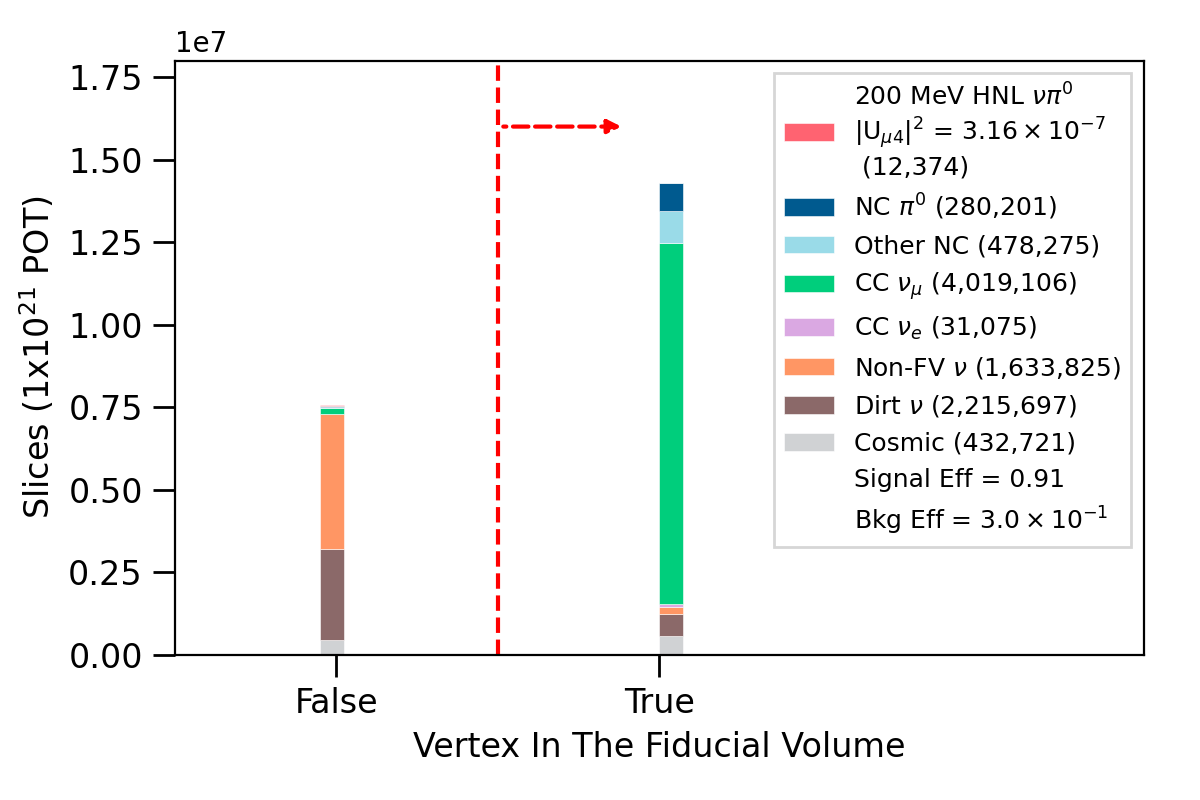
\includegraphics[width=\textwidth]{fv_precut}
            \caption{Fiducial volume cut}%
            \label{fig:fv_cut}
        \end{subfigure}
        \hfill
        \begin{subfigure}[b]{0.495\textwidth}   
            \centering 
            \includegraphics[width=\textwidth]{beam_bucket_post_fv}
            \caption{After fiducial volume cut}%
            \label{fig:bb_post_fv}
        \end{subfigure}
        \hfill
        \begin{subfigure}[b]{0.495\textwidth}   
            \centering 
            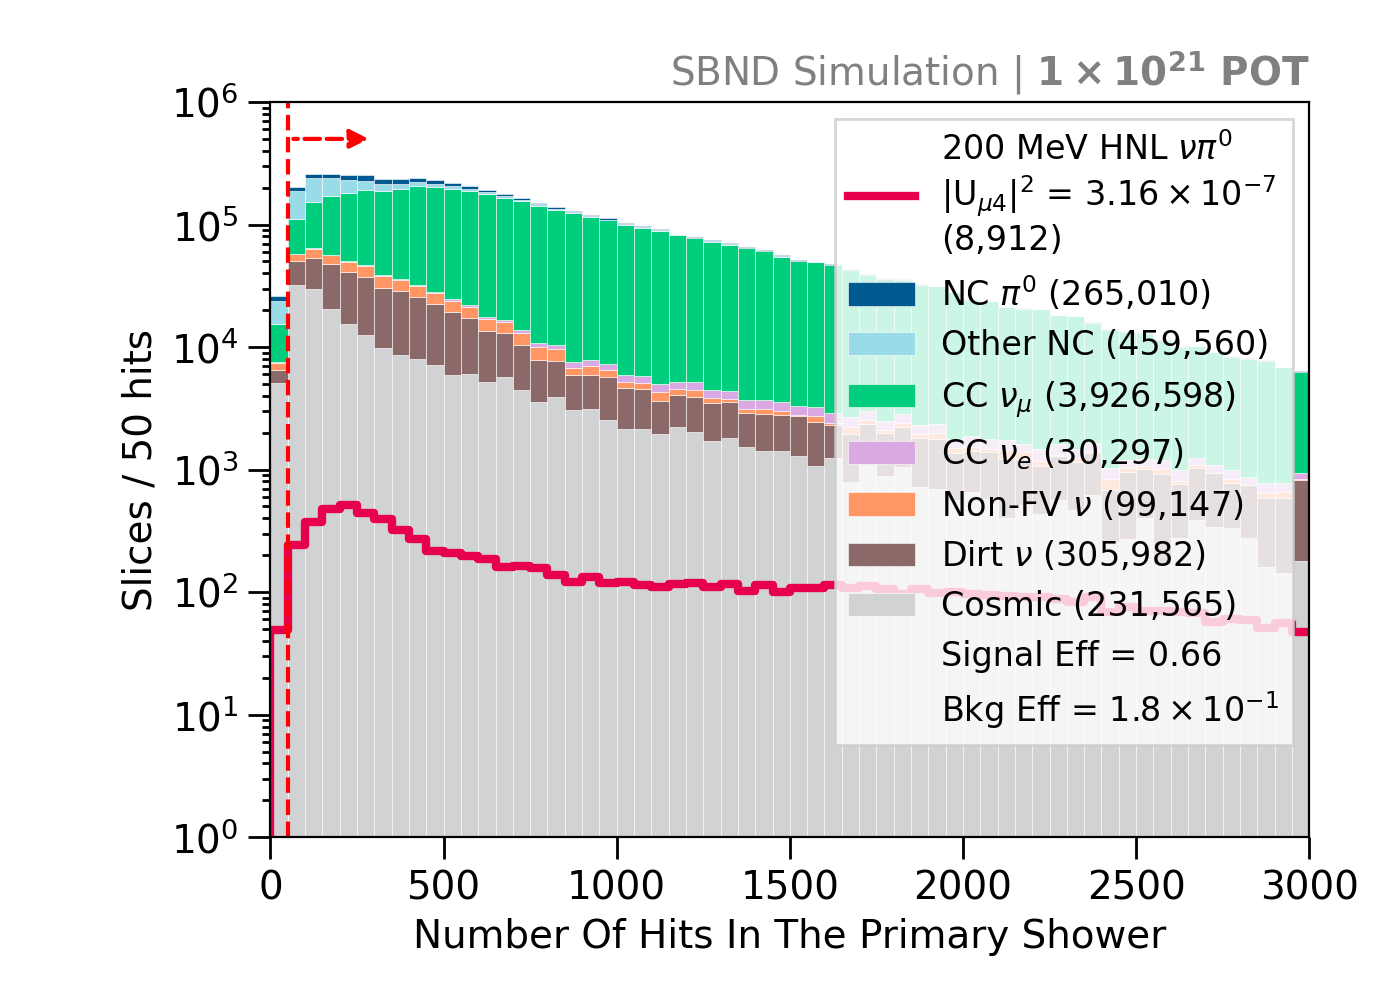
\includegraphics[width=\textwidth]{nHits}
            \caption{After number of hits cut}%
            \label{fig:Nhits_cut}
        \end{subfigure}
        \hfill
        \begin{subfigure}[b]{0.495\textwidth}   
            \centering 
            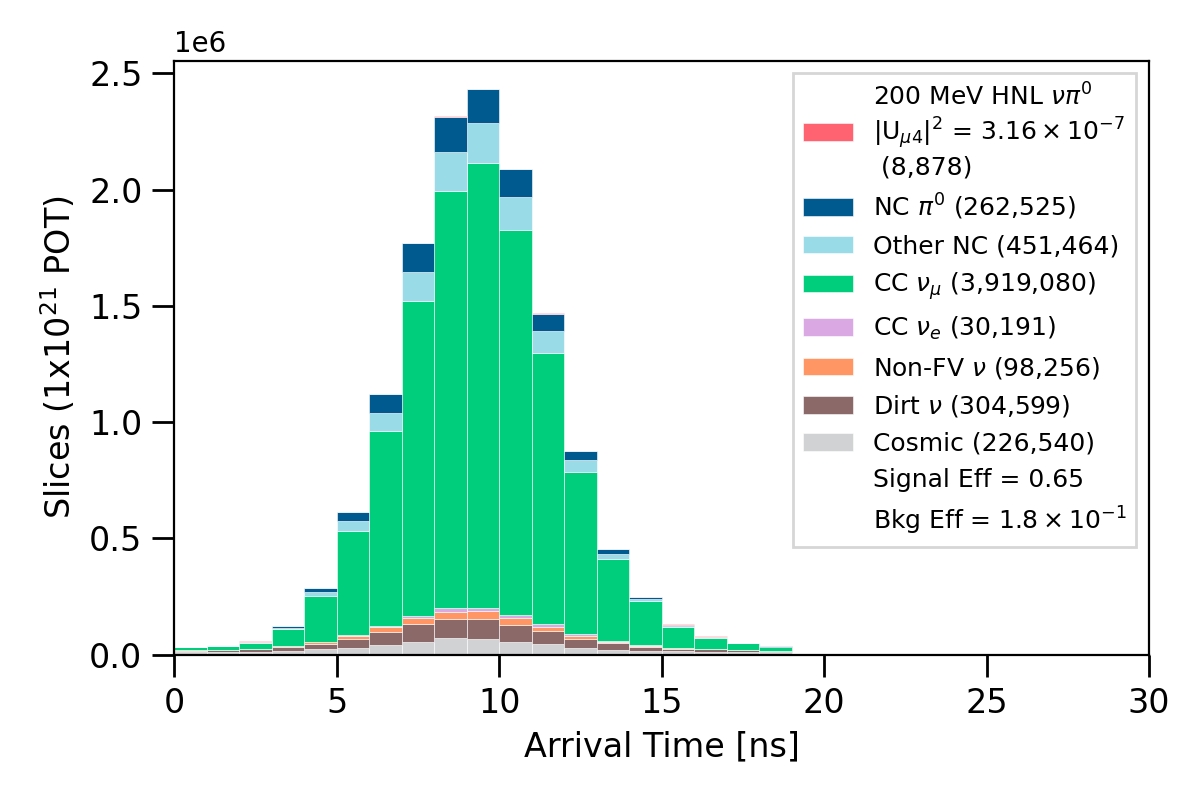
\includegraphics[width=\textwidth]{beam_bucket_postNhits}
            \caption{After number of hits cut}%
            \label{fig:bb_postNhits}
        \end{subfigure}
        \caption{
		Plots demonstrating the FV and number of hits cuts (left column) and the resulting beam bucket distribution after each cut (right column). 
	}
        \label{fig:quality_cut}
\end{figure}

\subsection{SM Neutrino Track Removal}

The next sets of cuts focus on rejecting SM neutrino backgrounds that produce tracks originating from muons, protons and pions.
The cut uses the score distribution from the Razzled BDT, previously detailed in Sec. \ref{sec:razzled}.
There are two types of Razzled variables examined for this cut: (1) the number of particle-type in a slice as identified by Razzled and (2) the Razzled particle-type scores of particles in a slice.
The former cut relies on Razzled assigning a type to a particle based on its highest particle-type score from the BDT.
The latter cut is to further reject slices if they contain particles with a Razzled score higher than a chosen threshold.

Fig. \ref{fig:nrazzled_muon_full} and \ref{fig:razzled_muon_score_full} demonstrate the two cuts respectively for rejecting muon-like particles.
Fig. \ref{fig:nrazzled_muon_full} shows the requirement on the number of Razzled-identified muons is 0 while Fig. \ref{fig:razzled_muon_score_full} shows that only slices containing particles with Razzled muon score $< 0.04$ are selected.
The cuts are very aggressive without comprising signal efficiency due to the distinction between HNL signals and muon tracks.  
Comparison between the beam bucket distribution before and after the muon cut, Fig. \ref{fig:bb_postNhits} and Fig. \ref{fig:bb_post_muon}, can be made to evaluate the impacts of the cut.
The muon cut effectively rejects $96\%$ of the $4$ million CC $\nu_\mu$ slices, leaving only $\sim161,000$ slices remaining.
HNL slices are also affected by the cut such that the signal efficiency reduces from 65\% to 51\%.

\begin{figure}[t!]
        \begin{subfigure}[b]{0.495\textwidth}   
            \centering 
            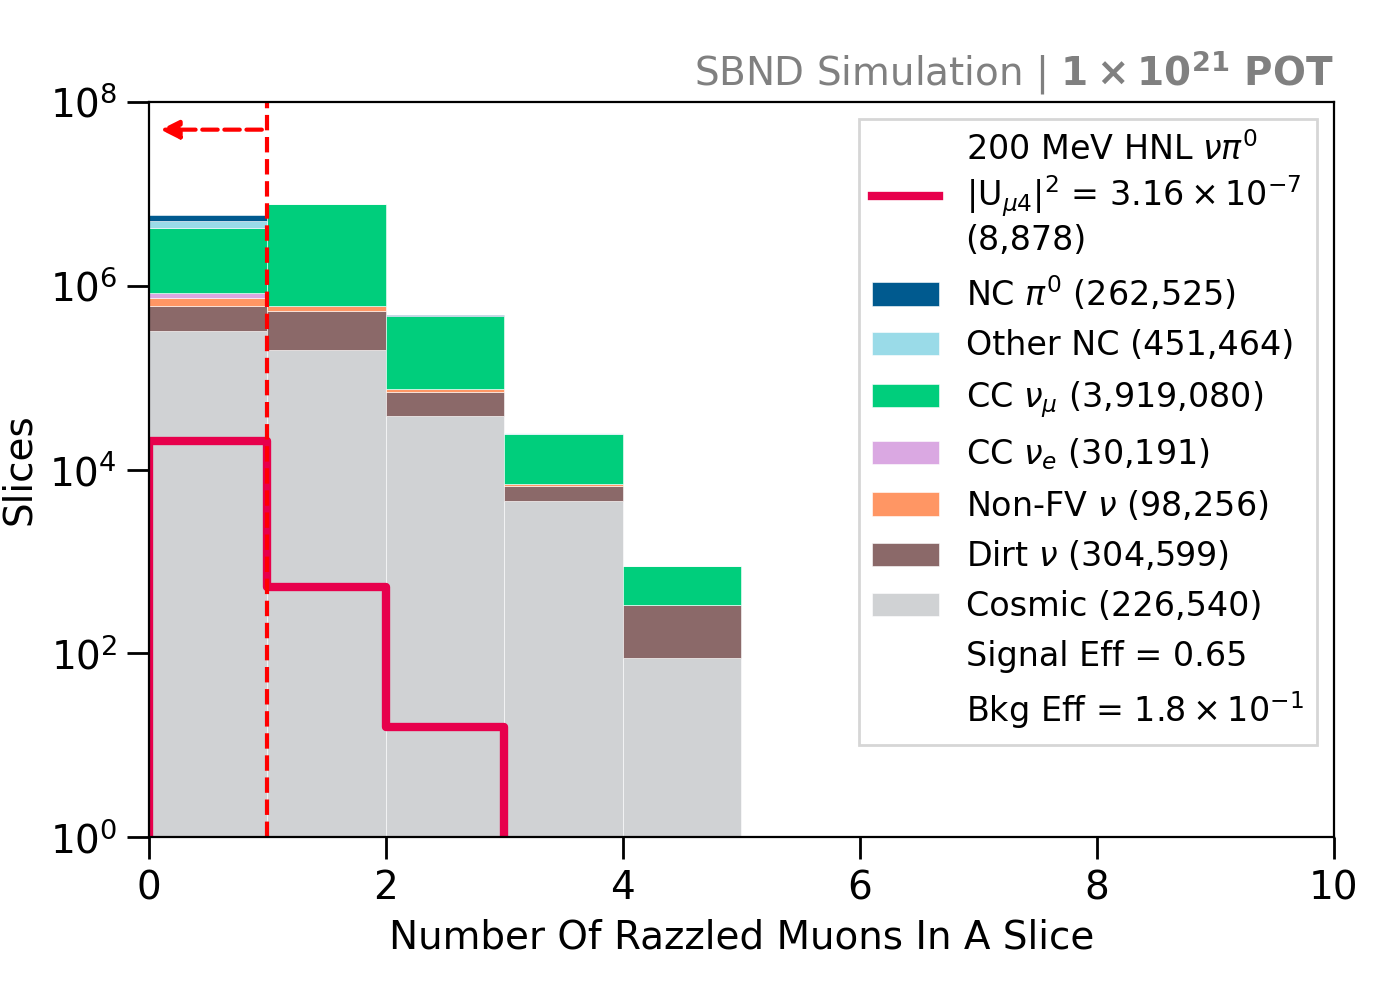
\includegraphics[width=\textwidth]{nrazzled_muon_precut}
            \caption{Number of Razzled-identified muons cut}%
            \label{fig:nrazzled_muon_full}
        \end{subfigure}
        \hfill
        \begin{subfigure}[b]{0.495\textwidth}   
            \centering 
            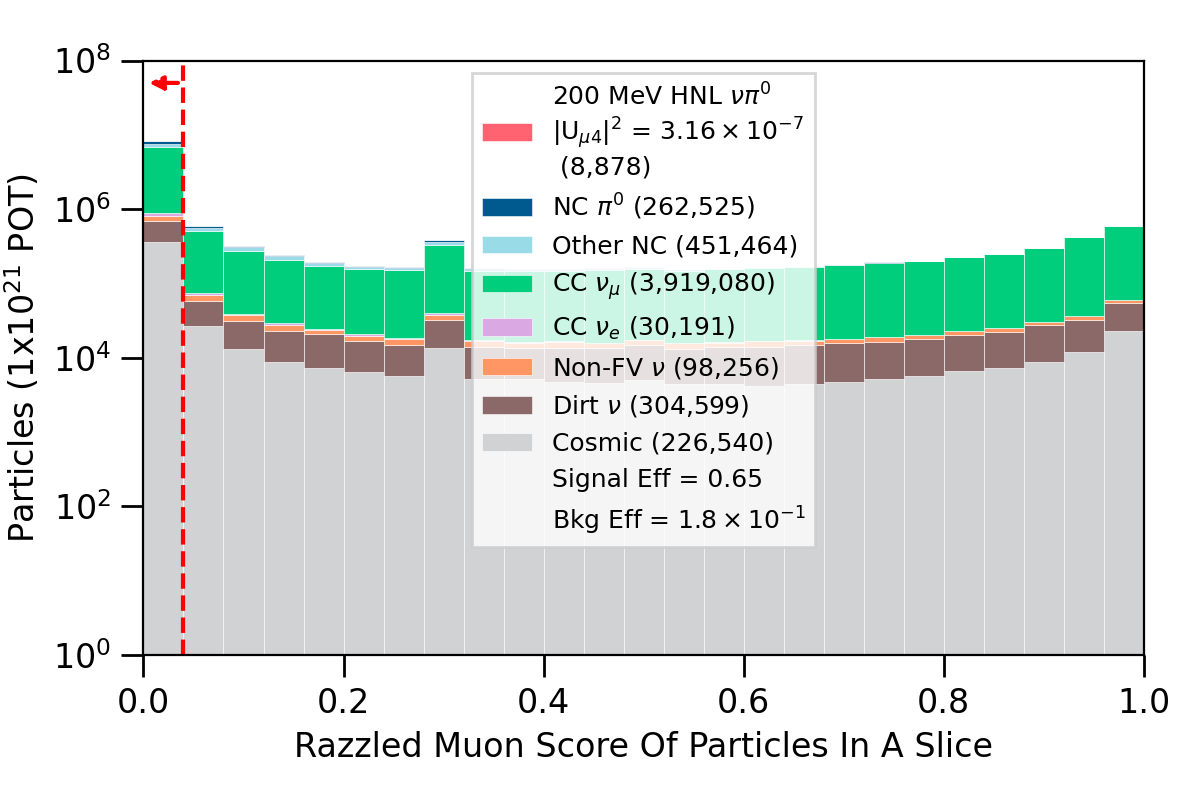
\includegraphics[width=\textwidth]{razzled_muon_score_precut}
            \caption{Particles with Razzled muon score cut}%
            \label{fig:razzled_muon_score_full}
        \end{subfigure}
        \hfill
	\centering
        \begin{subfigure}[b]{0.495\textwidth}   
            \centering 
            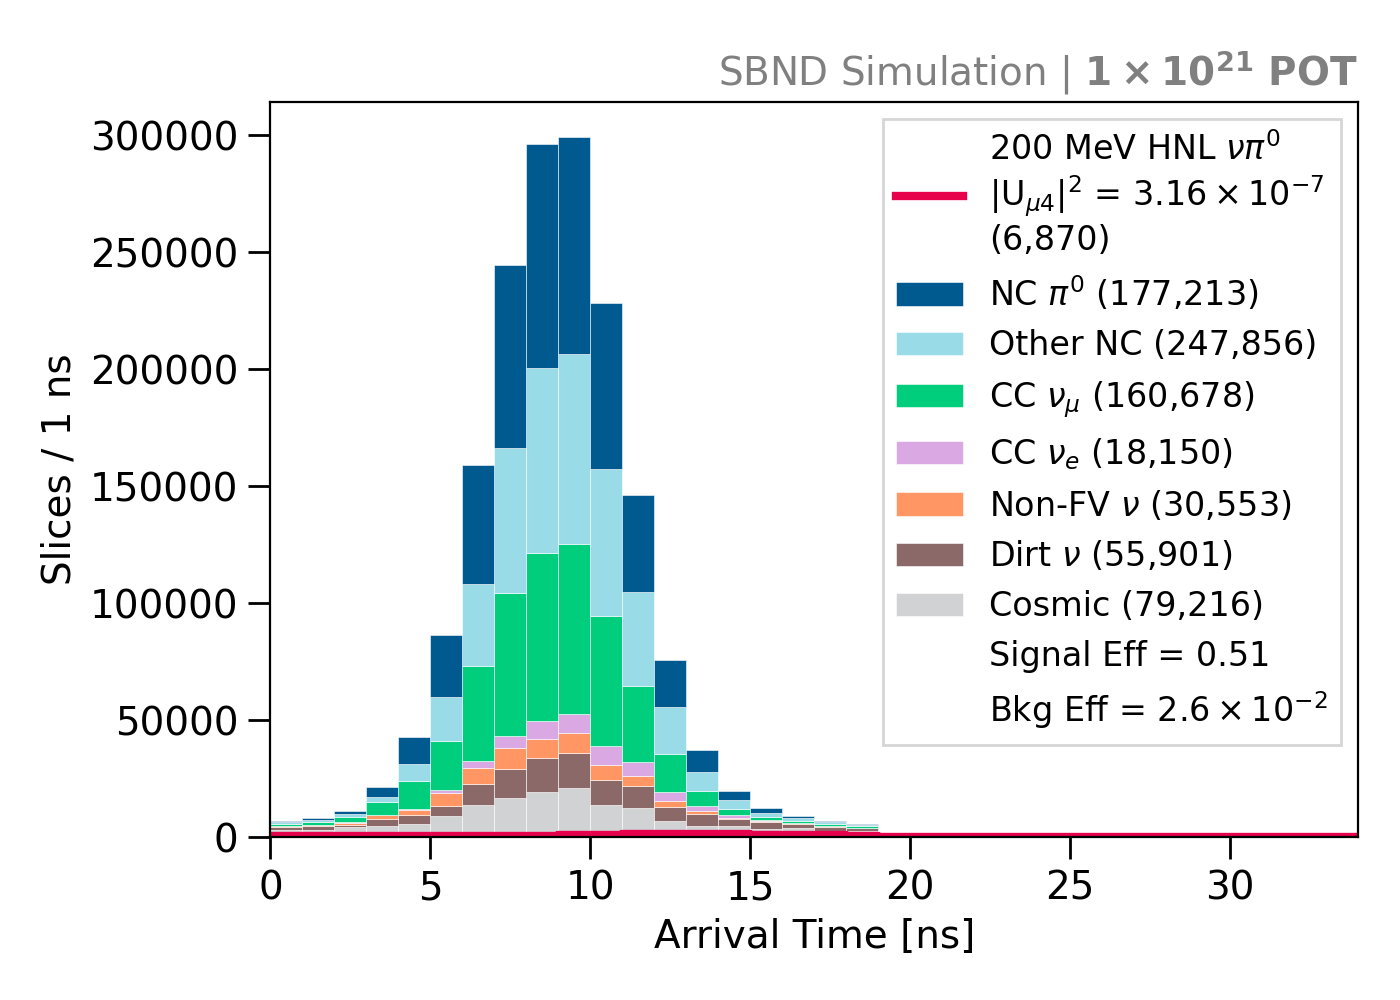
\includegraphics[width=\textwidth]{beam_bucket_postmuon}
            \caption{After muon cut}%
            \label{fig:bb_post_muon}
        \end{subfigure}
        \caption{
		Plots demonstrating the muon cuts (top) and the resulting beam bucket distribution after the cuts (bottom). 
	}
        \label{fig:razzled_muon_cut}
\end{figure}

Similar cuts are then applied consecutively to reject protons and pions, with thresholds on the Razzled score varying depending on the particle type.
Additional conditions are required on the reconstructed Kinetic Energy (KE) to be $ > 32.7$ MeV for protons and $< 32.1$ MeV for pions to ensure particles are well-reconstructed. 
To summarise, the cuts to reject muons, protons and pions are as follows
\begin{enumerate}
\item Muon cuts:
    \begin{coloritemize}
        \item Number of Razzled-identified muons in a slice = 0
        \item Slices containing only particles with Razzled muon score $<$ 0.04
    \end{coloritemize}
\item Proton cuts:
    \begin{coloritemize}
        \item Number of Razzled-identified protons with KE $>$ 32.7 MeV in a slice = 0
        \item Slices containing only particles with Razzled proton score $<$ 0.96
    \end{coloritemize}
\item Pion cuts:
    \begin{coloritemize}
        \item Number of Razzled-identified pions KE $>$ 32.1 MeV in a slice = 0
        \item Slices containing only particles with Razzled pion score $<$ 0.82
    \end{coloritemize}
\end{enumerate}
\begin{figure}[b!]
        \begin{subfigure}[b]{0.495\textwidth}   
            \centering 
            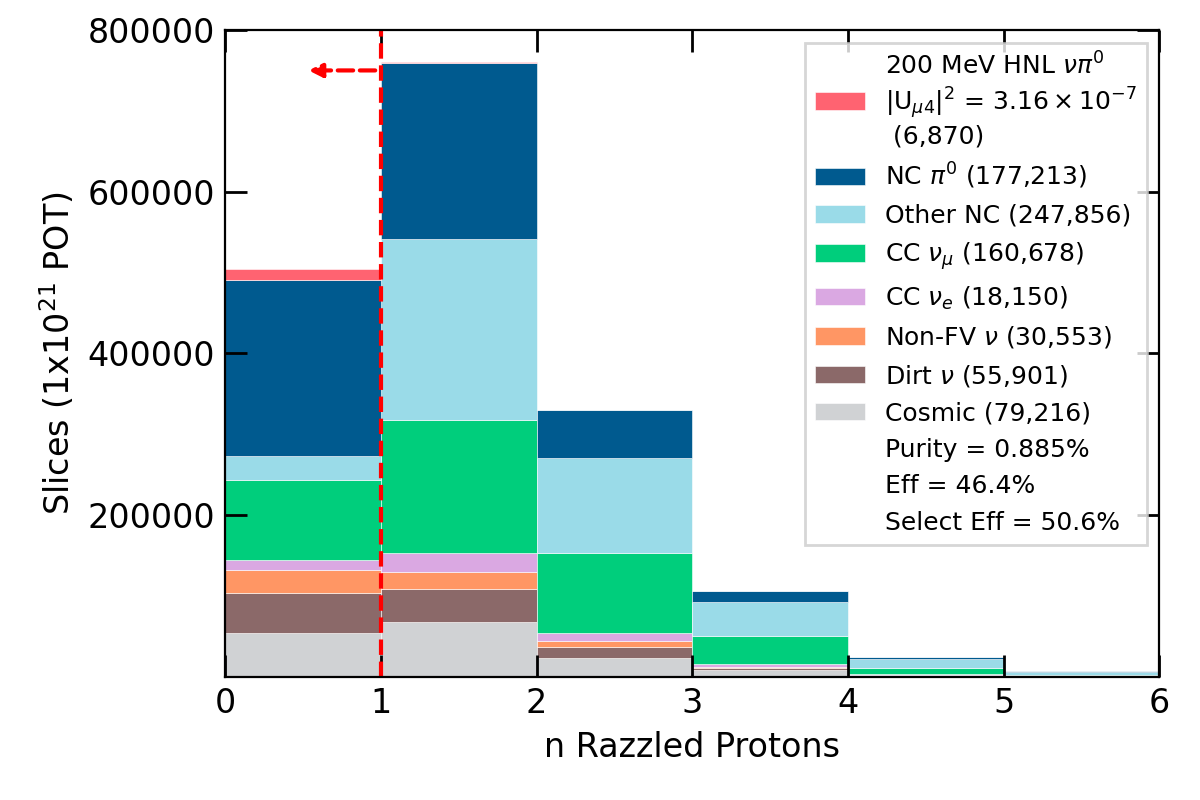
\includegraphics[width=\textwidth]{nrazzled_proton_precut}
            \caption{Number of Razzled-identified protons cut}%
            \label{fig:nrazzled_proton_full}
        \end{subfigure}
        \hfill
        \begin{subfigure}[b]{0.495\textwidth}   
            \centering 
            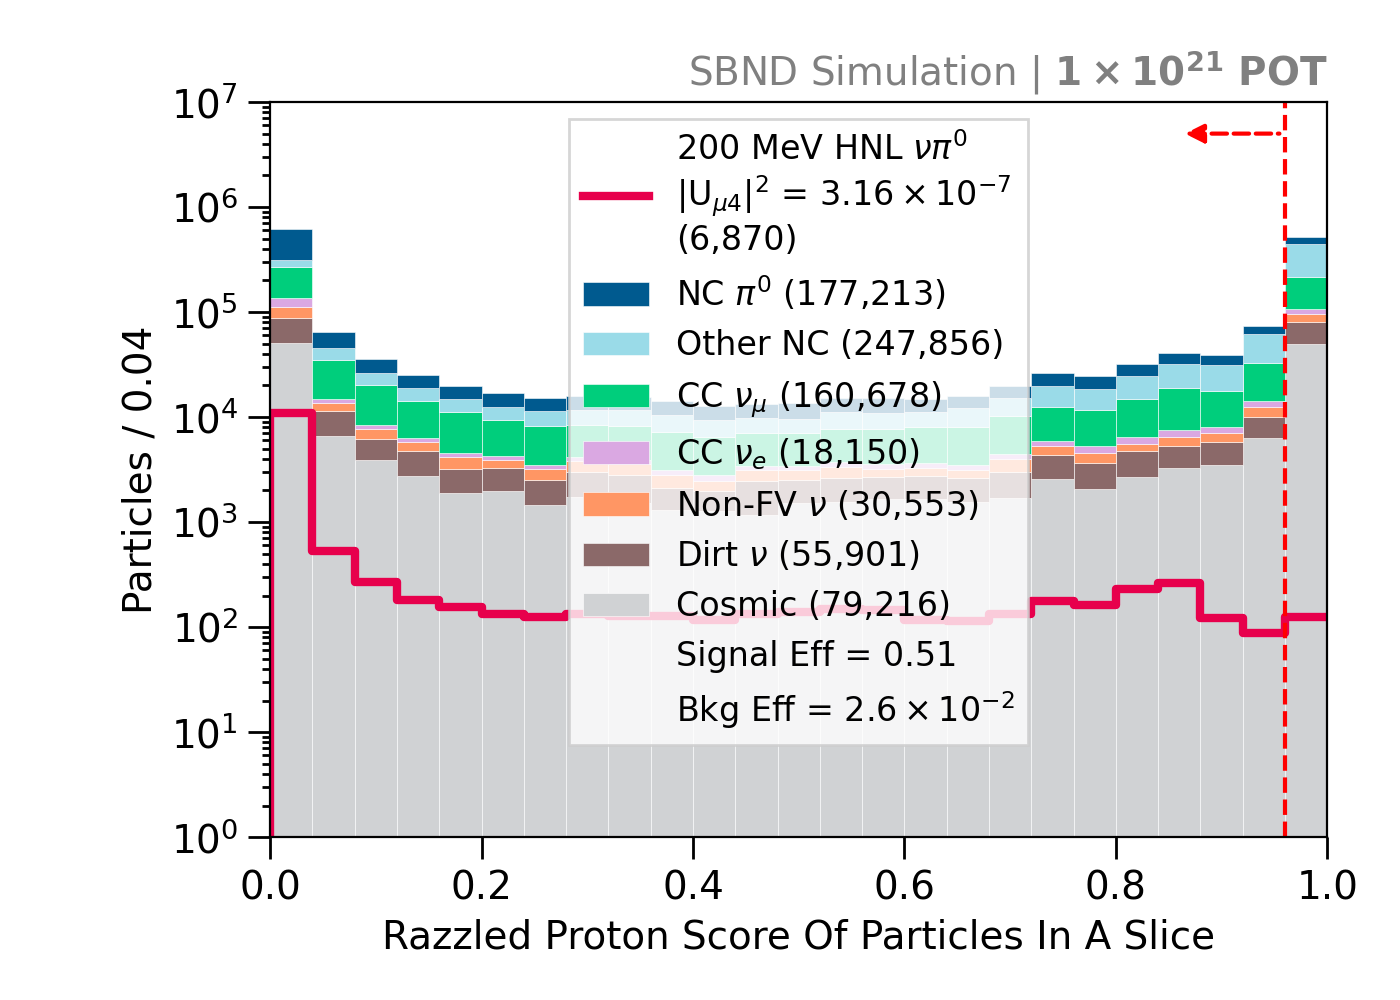
\includegraphics[width=\textwidth]{razzled_proton_score_precut}
            \caption{Particles with Razzled proton score cut}%
            \label{fig:razzled_proton_score_full}
        \end{subfigure}
        \hfill
	\centering
        \begin{subfigure}[b]{0.495\textwidth}   
            \centering 
            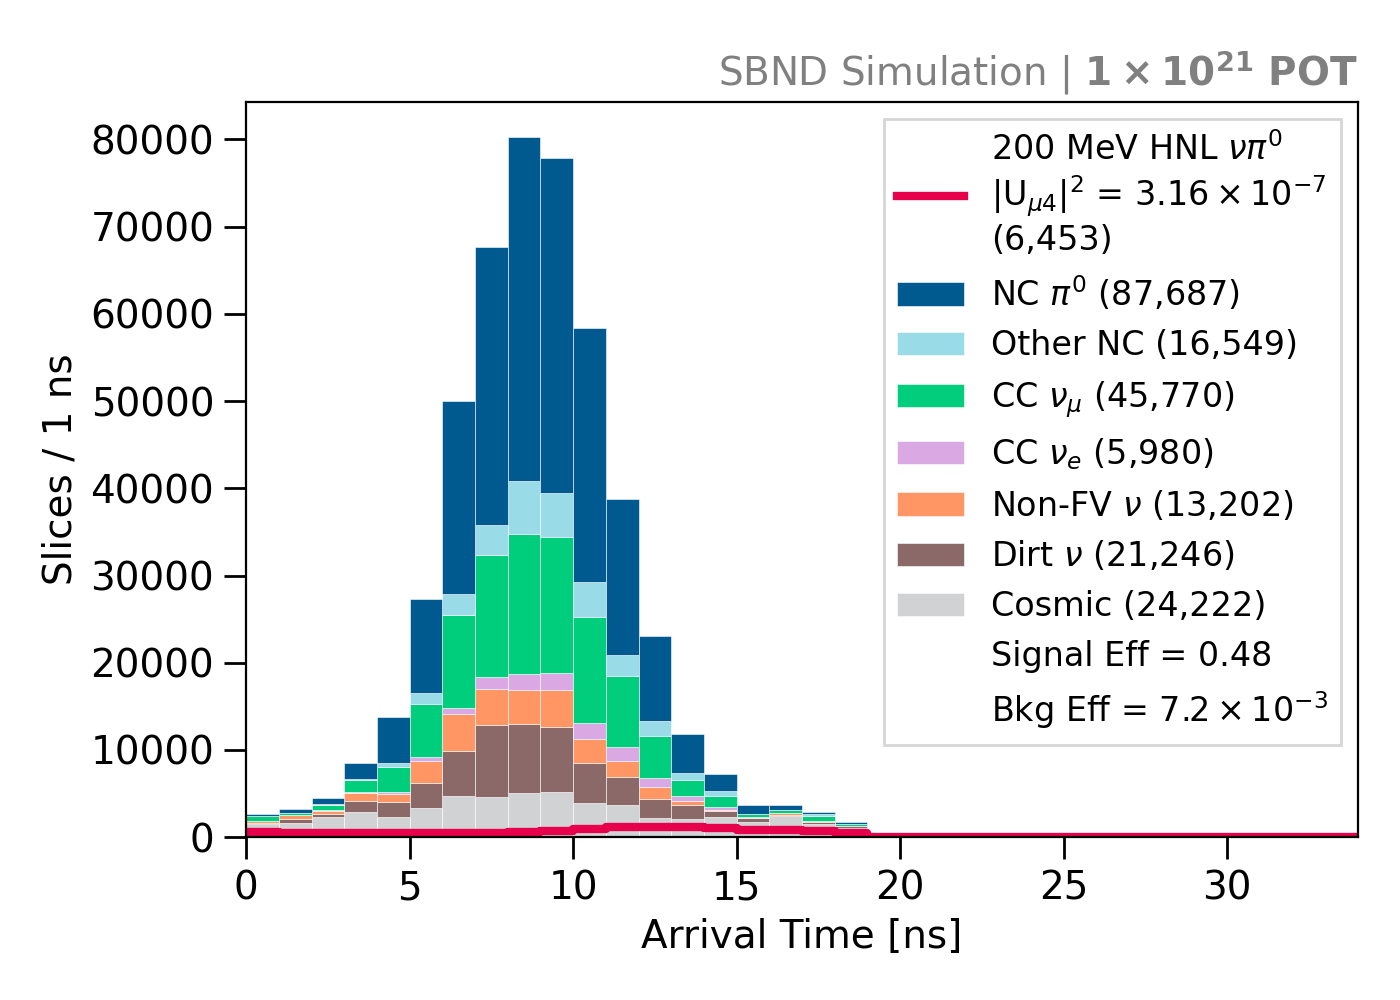
\includegraphics[width=\textwidth]{beam_bucket_postproton}
            \caption{After proton cut}%
            \label{fig:bb_post_proton}
        \end{subfigure}
        \caption{
		Plots demonstrating the proton cuts (top) and the resulting beam bucket distribution after the cuts (bottom). 
	}
        \label{fig:razzled_proton_cut}
\end{figure}
The cuts to reject protons and pions are demonstrated in Fig. \ref{fig:razzled_proton_cut} and \ref{fig:razzled_pion_cut} respectively.
Similarly to the muon cut, these cuts are also very aggressive to require that the selected slices not contain any track-like particles.
The impacts of the proton cut can be seen in the beam bucket distribution in Fig. \ref{fig:bb_post_proton}, as any interactions producing protons are removed, significantly reducing SM neutrino backgrounds.
The most impacted interaction modes are Other NC interactions reducing from $\sim249,000$ to $\sim17,000$ slices, CC $\nu_\mu$ interactions reducing from $\sim161,000$ to $\sim46,000$ slices and NC $\pi^0$ interactions reducing from $\sim 177,000$ to $\sim88,000$ slices.
The result of the pion cut can be observed in the beam bucket distribution shown in Fig. \ref{fig:bb_post_pion}, where the cut further cleans up any SM neutrino slices that are not already rejected by the muon and proton cut.  
The background rejection efficiency at the end of the track removal significantly increases by two orders of magnitudes from $\mathcal{O}(10^{-1})$ to $\mathcal{O}(10^{-3})$.
Meanwhile, the HNL signal efficiency only decreases by 65\% to 46\%.

\begin{figure}[h!]
        \begin{subfigure}[b]{0.495\textwidth}   
            \centering 
            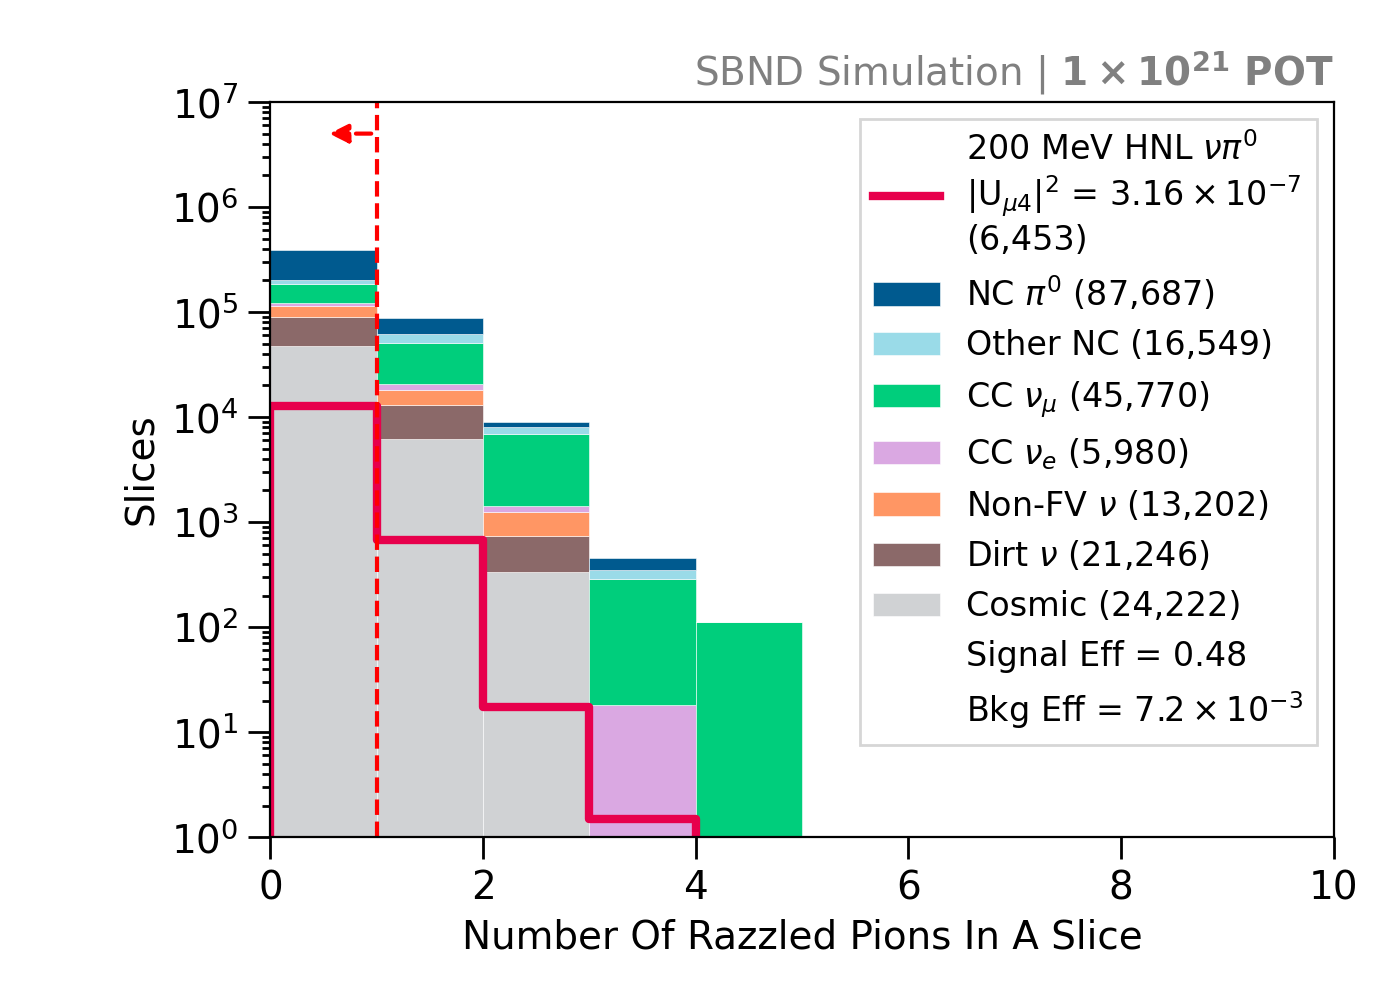
\includegraphics[width=\textwidth]{nrazzled_pion_precut}
            \caption{Number of Razzled-identified pions cut}%
            \label{fig:nrazzled_pion_full}
        \end{subfigure}
        \hfill
        \begin{subfigure}[b]{0.495\textwidth}   
            \centering 
            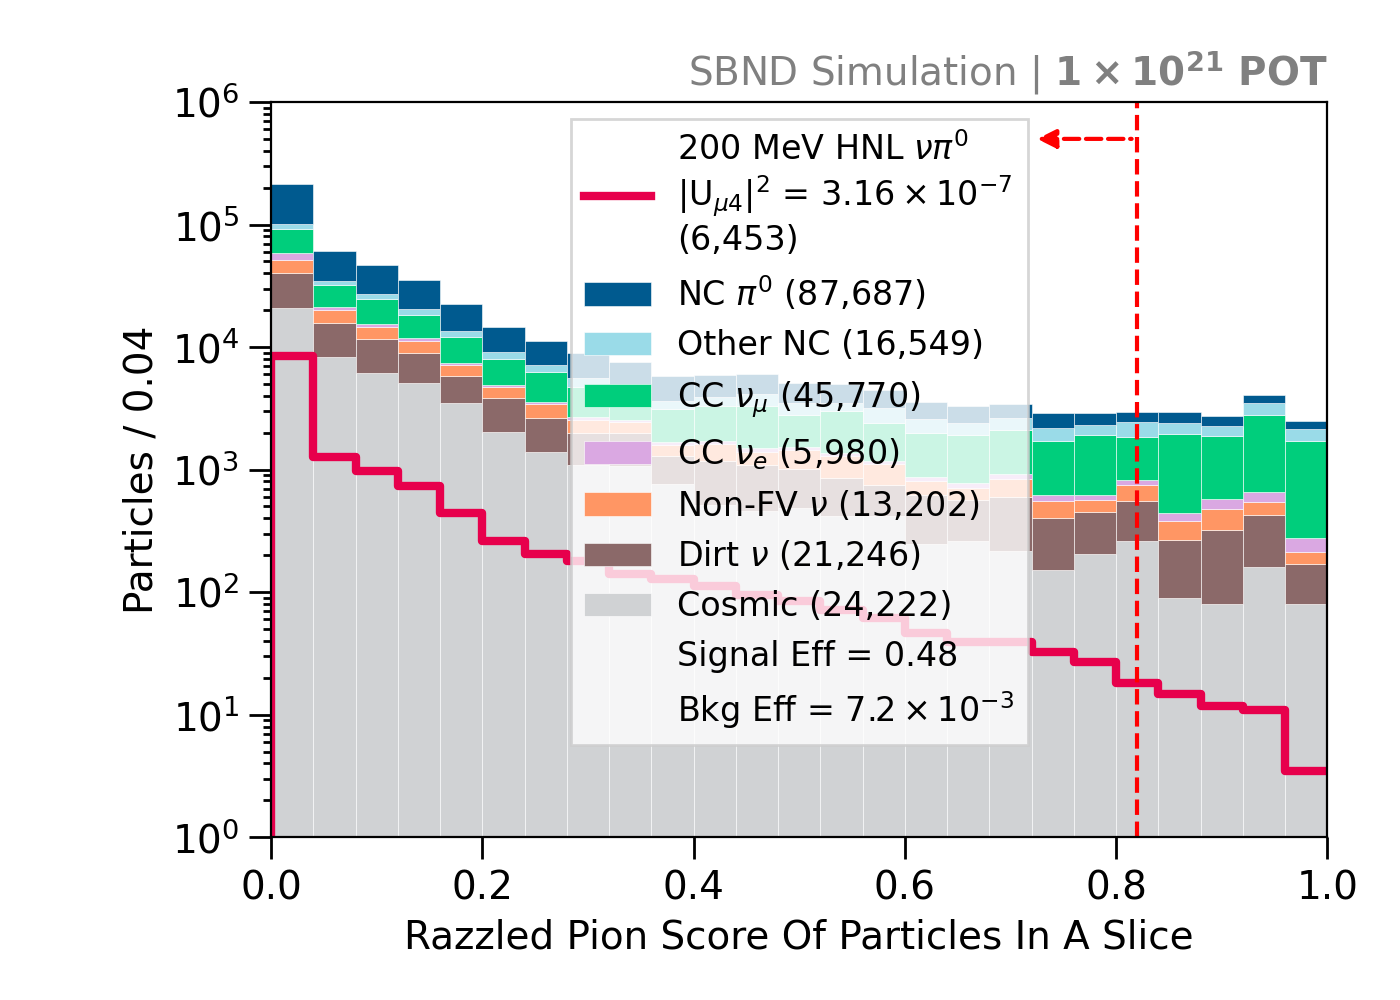
\includegraphics[width=\textwidth]{razzled_pion_score_precut}
            \caption{Particles with Razzled pion score cut}%
            \label{fig:razzled_pion_score_full}
        \end{subfigure}
        \hfill
	\centering
        \begin{subfigure}[b]{0.495\textwidth}   
            \centering 
            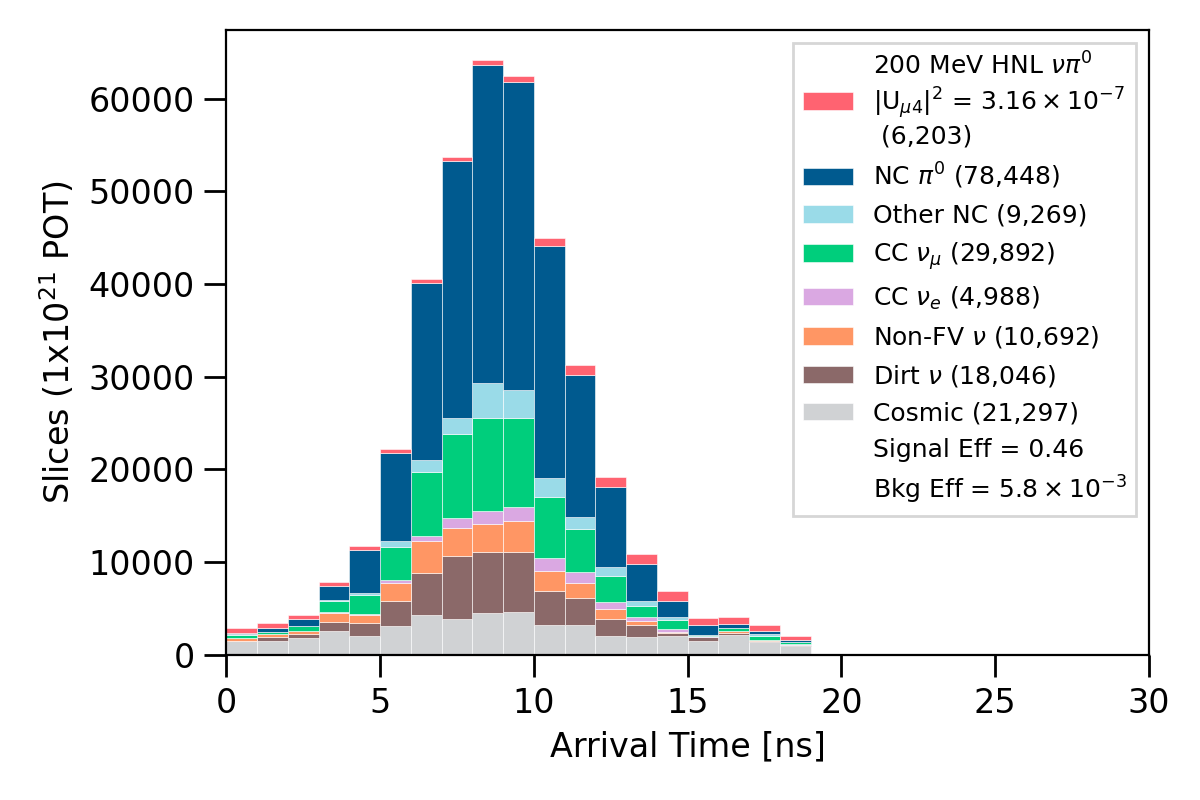
\includegraphics[width=\textwidth]{beam_bucket_postpion}
            \caption{After pion cut}%
            \label{fig:bb_post_pion}
        \end{subfigure}
        \caption{
		Plots demonstrating the pion cuts (top) and the resulting beam bucket distribution after the cuts (bottom). 
	}
        \label{fig:razzled_pion_cut}
\end{figure}
%********************************** %First Section  **************************************
\section{HNL Shower Selection}
\label{sec:hnl_shower_select}

\subsection{Electron Shower Removal}
%The resulting beam bucket distribution after the track removal can be seen in Fig. \ref{fig:bb_post_pion}, likely contains only interactions producing showers at this stage.
%The first dominated background is from NC $\pi^0$ interactions producing di-photon showers.
%%TODO: check this statement
%This is followed by CC $\nu_\mu$ interactions likely by deep inelastic scattering producing shower-like daughter particles.
%Another dominated background is from Non-FV and dirt neutrino combined, likely by the same interaction modes with daughter products propagate and deposit energy inside the detector.

After the track removal, the next sets of cuts target specifically at identifying HNL showers from trickier shower-like backgrounds.
The first cut of this HNL shower selection aims at rejecting showers originating from electrons.
The key differences between electron showers and photon showers are the shower conversion gap and the shower dE/dx.
The conversion gap describes the gap between the interaction vertex and the start of the shower, where electron showers start immediately at the vertex but photon showers might propagate away from the vertex before showering. 
The dE/dx describes the charge distribution per unit length such that the dE/dx of a photon shower is twice of an electron shower since a photon shower is made up of a pair of electron-positron showers.
Both these shower characteristics are provided during the training of the Razzled BDT for classifying photons and electrons. 

The Razzled electron score is examined for the primary shower that deposits the most energy in a slice.
The cut is demonstrated in Fig. \ref{fig:razzled_electron_cut}, where only slices containing primary showers with a Razzled electron score $< 0.96$ are selected.
This is a very soft cut compared to the previous track removal cuts since showers from CC $\nu_e$ interactions and showers from HNLs are very similar to each other.
Thus, only clearly-identified CC $\nu_e$ showers with high Razzled electron scores are removed.
The cut rejects $31\%$ of the remaining $\sim5,000$ CC $\nu_e$ slices while minimally reduces HNL slices by only $3 \%$.

\begin{figure}[htbp!]
        \begin{subfigure}[b]{0.495\textwidth}   
            \centering 
            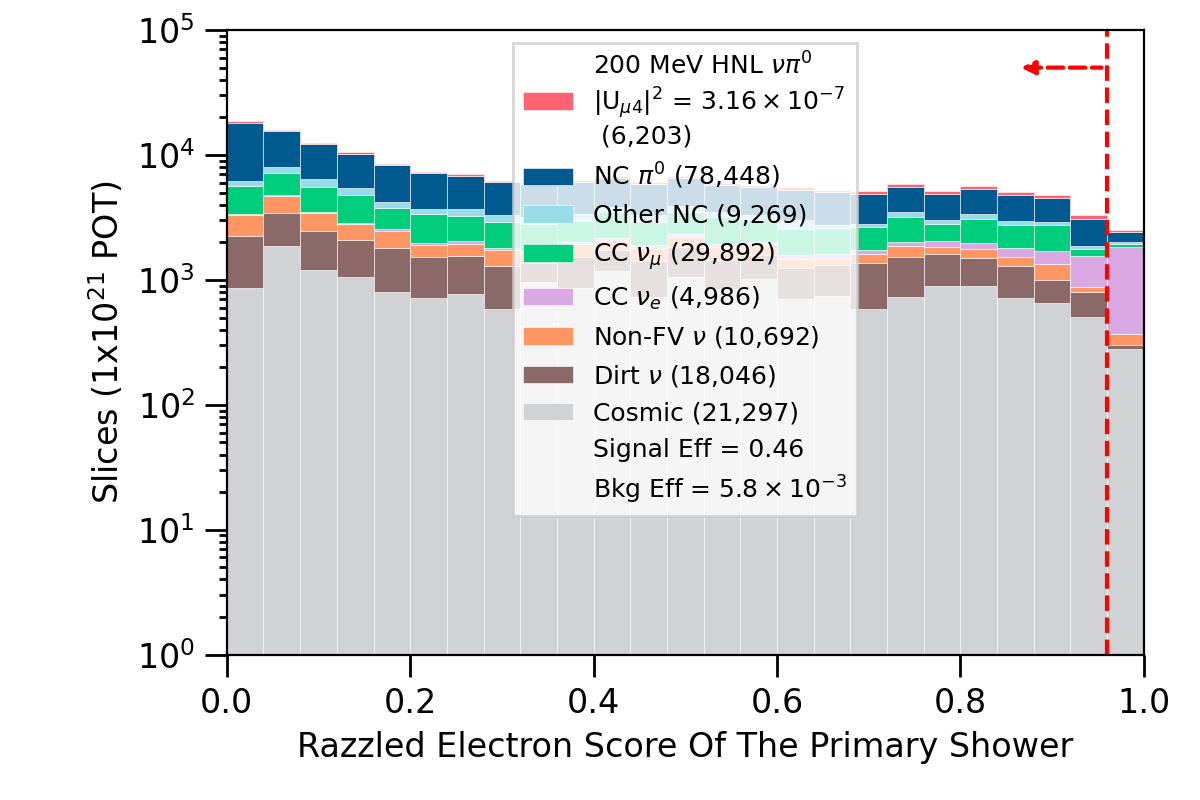
\includegraphics[width=\textwidth]{razzled_electron_score_prim_shw_precut}
            \caption{Primaries with Razzled electron score cut}%
            \label{fig:nrazzled_electron_full}
        \end{subfigure}
        \hfill
        \begin{subfigure}[b]{0.495\textwidth}   
            \centering 
            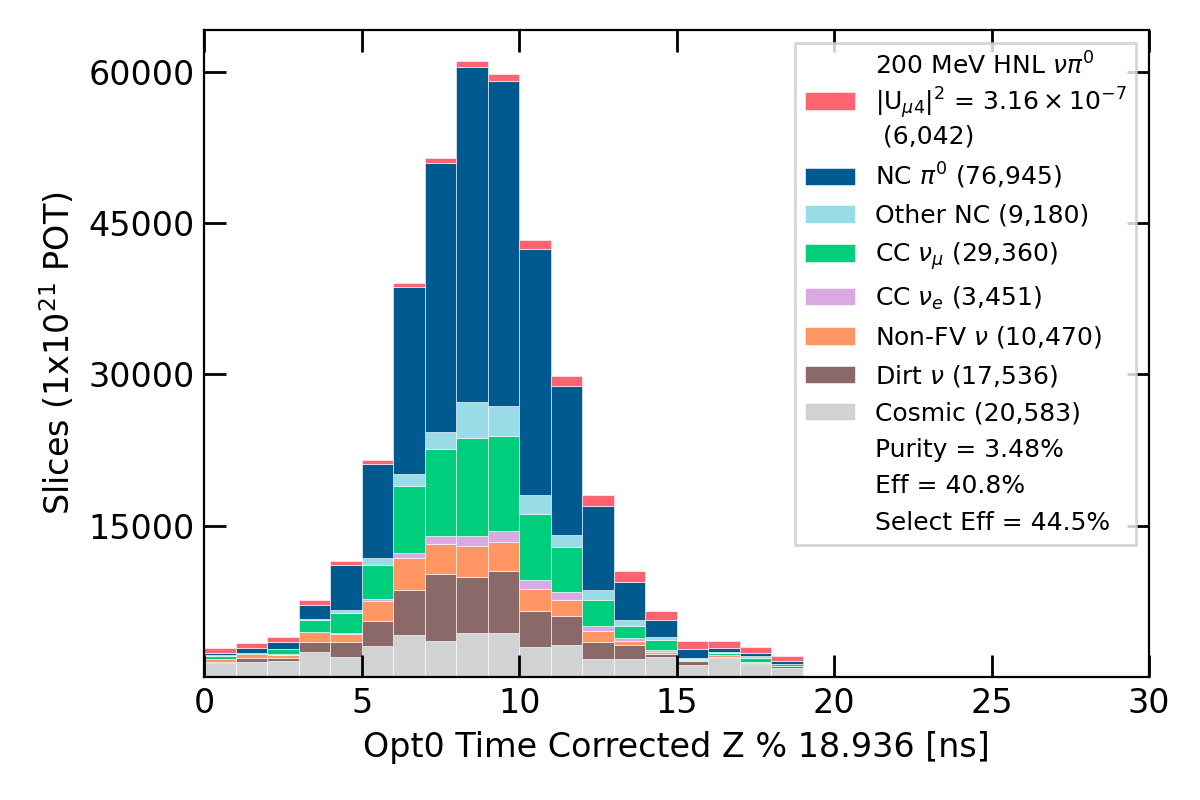
\includegraphics[width=\textwidth]{beam_bucket_postelectron}
            \caption{After electron cut}%
            \label{fig:bb_post_electron}
        \end{subfigure}
        \caption{
		Plots demonstrating the electron cut (top) and the resulting beam bucket distribution after the cut (bottom). 
	}
        \label{fig:razzled_electron_cut}
\end{figure}
%********************************** %First Section  **************************************
\subsection{Track Score Cut}

%The next set of cut after SM neutrinos removal focus on identifying HNL showers from the trickier background from SM NC $\pi^0$ interactions.
To further reject backgrounds containing showers, careful considerations were taken into developing cuts by separating the shower topology into subsets.
As previously stated, di-photon showers from HNLs can result in either a single shower topology or multiple shower topology.
Thus, two cases can be considered when applying cuts: (1) Slices containing only one shower and (2) Slices containing two or more showers.
Signal and background slices distribute differently in the phase space of the cut variable between the two cases, resulting in a different signal-to-background ratio.
From this cut onwards, individual cut is examined for each case to optimise the efficiency of background rejection and signal selection. 

\begin{figure}[b!]
        \begin{subfigure}[b]{0.495\textwidth}   
            \centering 
            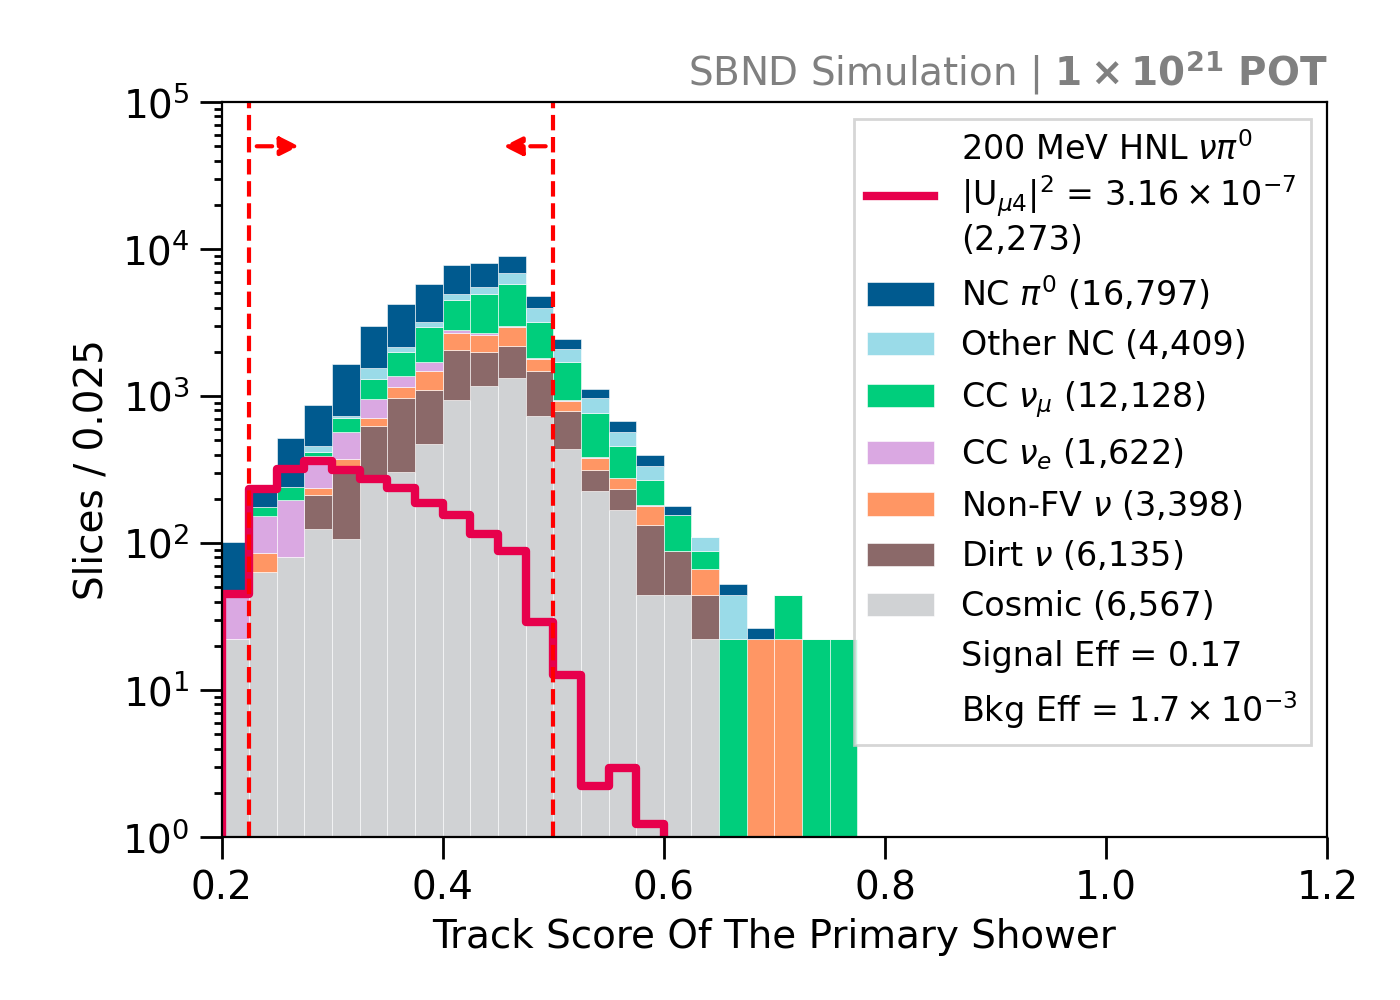
\includegraphics[width=\textwidth]{one_shw_track_score}
            \caption{1 Shower Case: Track score cut}%
        \end{subfigure}
        \hfill
        \begin{subfigure}[b]{0.495\textwidth}   
            \centering 
            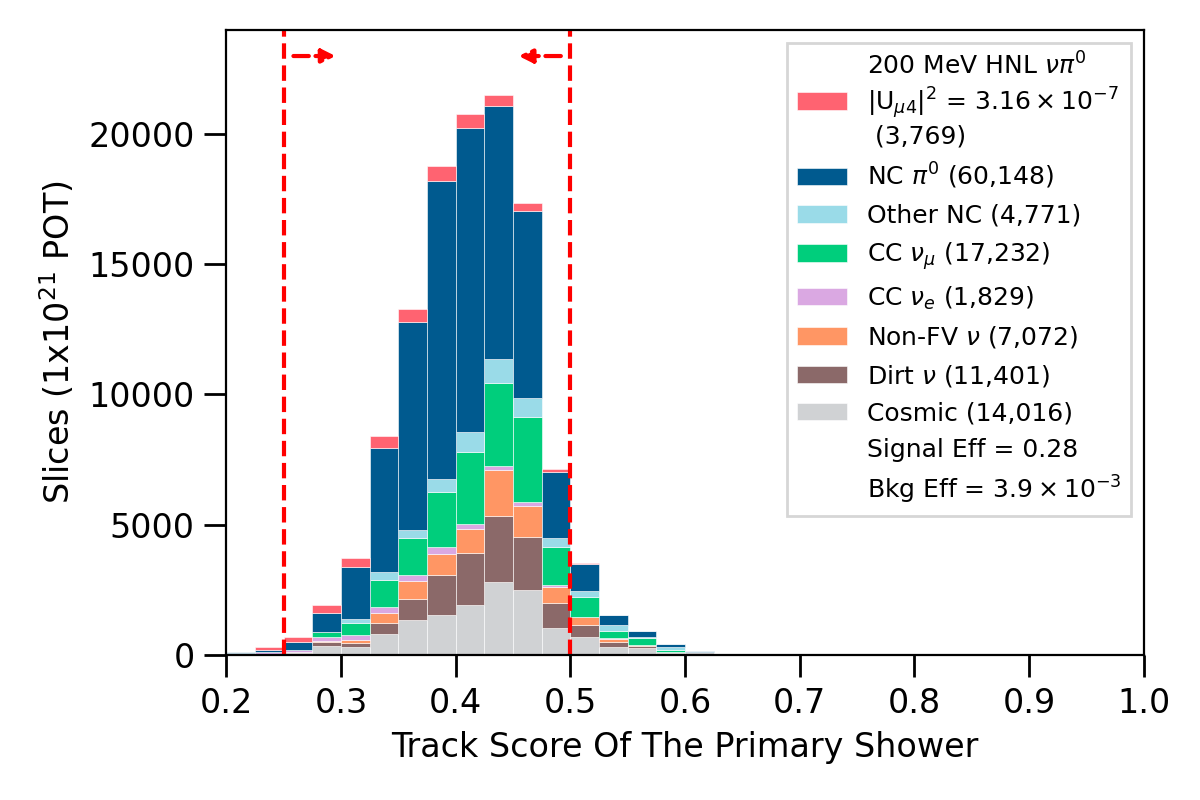
\includegraphics[width=\textwidth]{two_shower_primary_track_score_precut}
            \caption{2+ Showers Case: Track score cut}%
        \end{subfigure}
        \hfill
	\centering
        \begin{subfigure}[b]{0.495\textwidth}   
            \centering 
            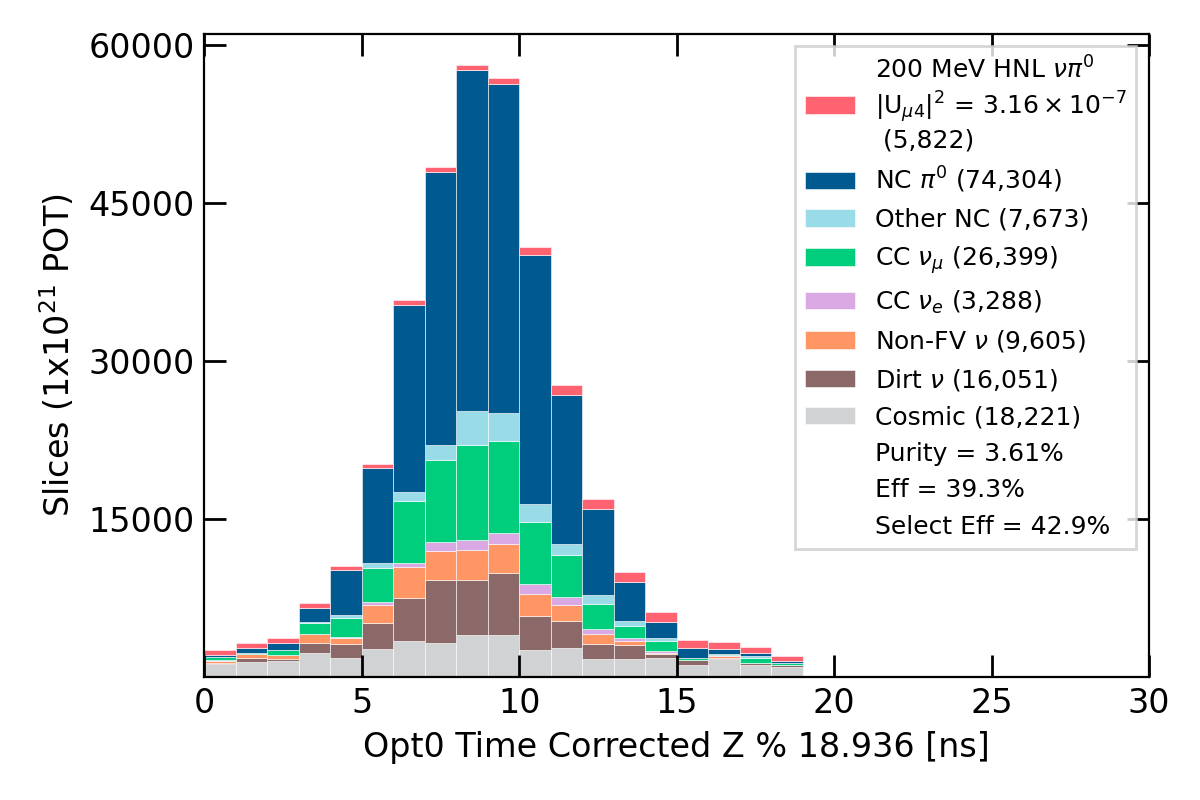
\includegraphics[width=\textwidth]{beam_bucket_postrackscore}
            \caption{After track score cut}%
	    \label{fig:bb_track_score}
        \end{subfigure}
        \caption{
		Plots demonstrating the track score cut (top) and the resulting beam bucket distribution after the cut (bottom). 
	}
        \label{fig:track_score_cut}
\end{figure}

The second cut of the HNL shower selection employs the track-shower separation BDT score, as previously discussed in Sec. \ref{sec:trkshwbdt}, to select only very-shower-like primaries.
Fig. \ref{fig:track_score_cut} displays the track score distribution of primary particles for the two cases of slices containing 1 shower and 2+ showers.
The remaining primary particles are already shower-like since the score concentrates in the region $< 0.5$.
For both cases, the track score is capped at 0.5 to reject any primary particles leaning towards track-like.
Comparing between the two cases, the signal-to-background ratio is higher across the score distribution the single shower case than the multiple showers case.
A more lenient cut is applied for the single shower case selecting the primary shower with a track score of $\geq 0.225$.
The cut is tightened up for the multiple showers case for better background rejection, requiring the primary shower to have a track score of $\geq 0.25$.
The resulting beam bucket distribution is depicted in Fig. \ref{fig:bb_track_score}, showing a reduction of $3\sim16\%$ across different SM neutrino interaction types.
Meanwhile, the signal selection efficiency minimally reduces from 45\% to 43\%.

\subsection{Calorimetry Cut}

The third cut of the HNL shower selection targets the highly energetic aspect of the showers resulting from HNL decays compared to SM neutrino showers.
Outputs from the flash-to-slice matching process are examined, as previously detailed in Sec. \ref{sec:subsystem_match}, particularly the fraction variable defined in Eq. \ref{eq:opt0fraction}.
As previously stated, the variable describes the level of agreement between hypothesis PE from reconstructed charge, $L_{\mathrm{Q}}$, and the measured PE seen by PMTs, $L$.
A large disagreement might indicate poor reconstruction, whether under or overestimation in light prediction or non-coincident cosmic backgrounds.
The fraction is useful to identify showers originating from HNLs due to their boosted topology.
Since HNL showers are forward-going, they are likely to overlap and be reconstructed as a shower merged from multiple showers.   
As a result, the reconstructed shower energy of HNLs using the measured charge tend to be much higher than SM neutrinos.
The number of PE predictions from the reconstructed energy, $L_{\mathrm{Q}}$, is therefore also likely to be overestimated compared to the measured PE seen by PMTs, $L$.

\begin{figure}[ht!]
        \begin{subfigure}[b]{0.495\textwidth}   
            \centering 
            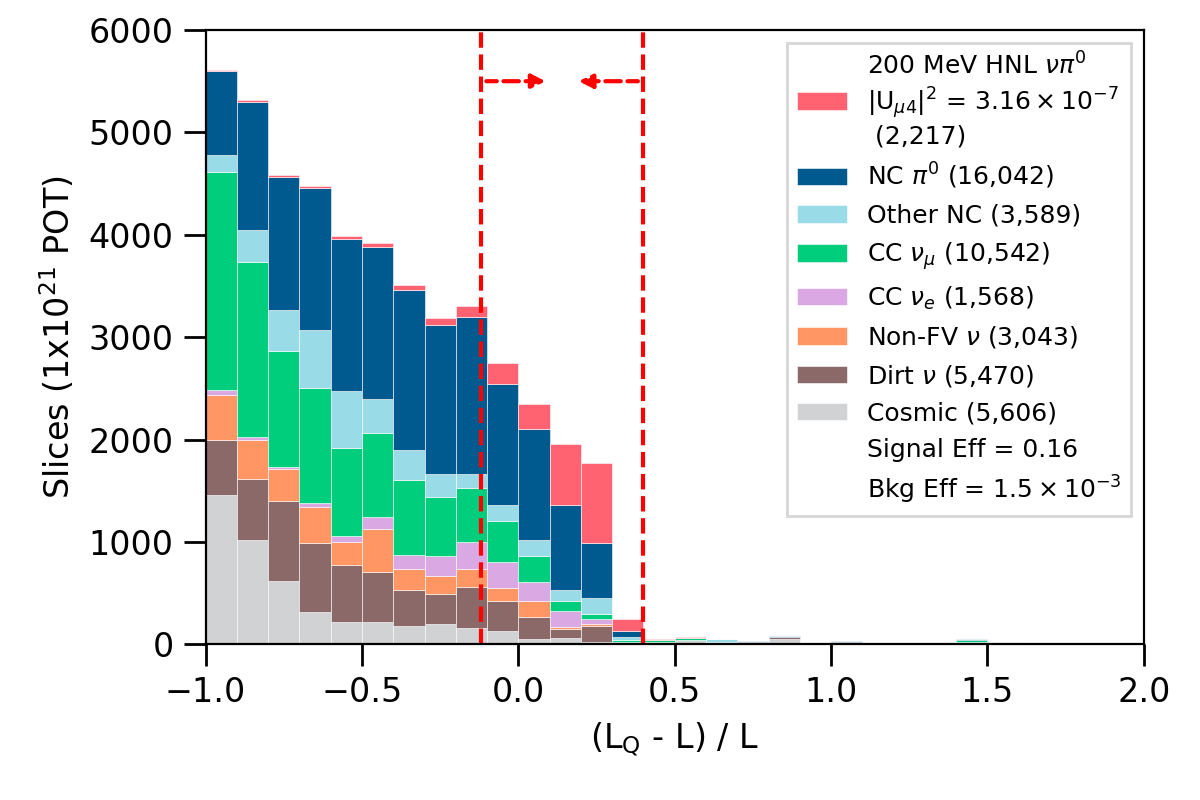
\includegraphics[width=\textwidth]{opt0frac_one_shw_precut}
            \caption{1 Shower Case: Calorimetry cut}%
        \end{subfigure}
        \hfill
        \begin{subfigure}[b]{0.495\textwidth}   
            \centering 
            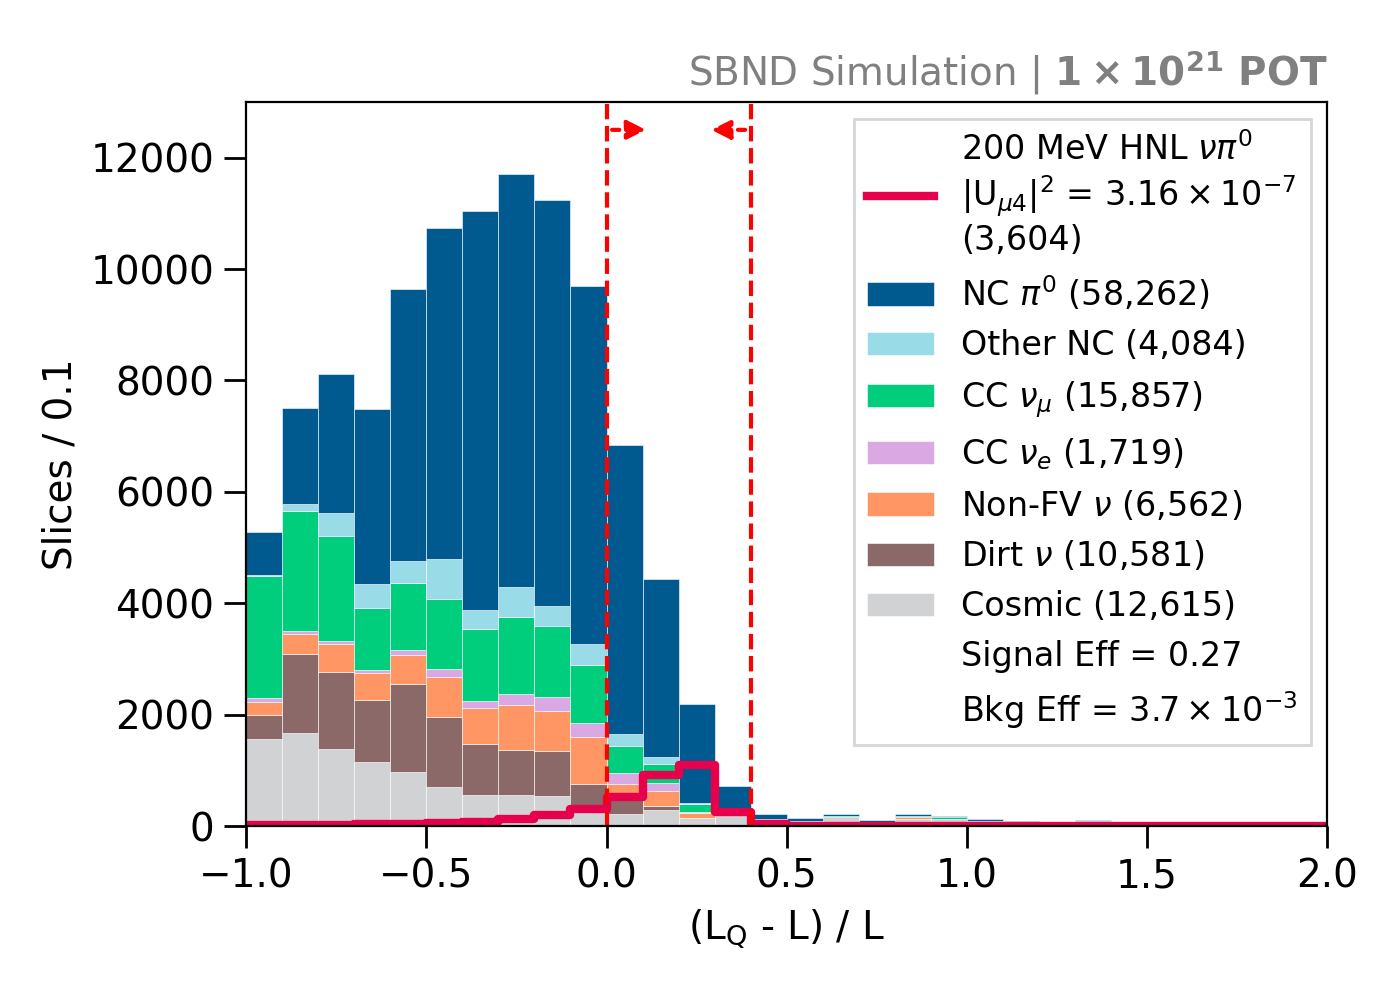
\includegraphics[width=\textwidth]{opt0frac_two_shw_precut}
            \caption{2+ Showers Case: Calorimetry cut}%
        \end{subfigure}
        \hfill
	\centering
        \begin{subfigure}[b]{0.495\textwidth}   
            \centering 
            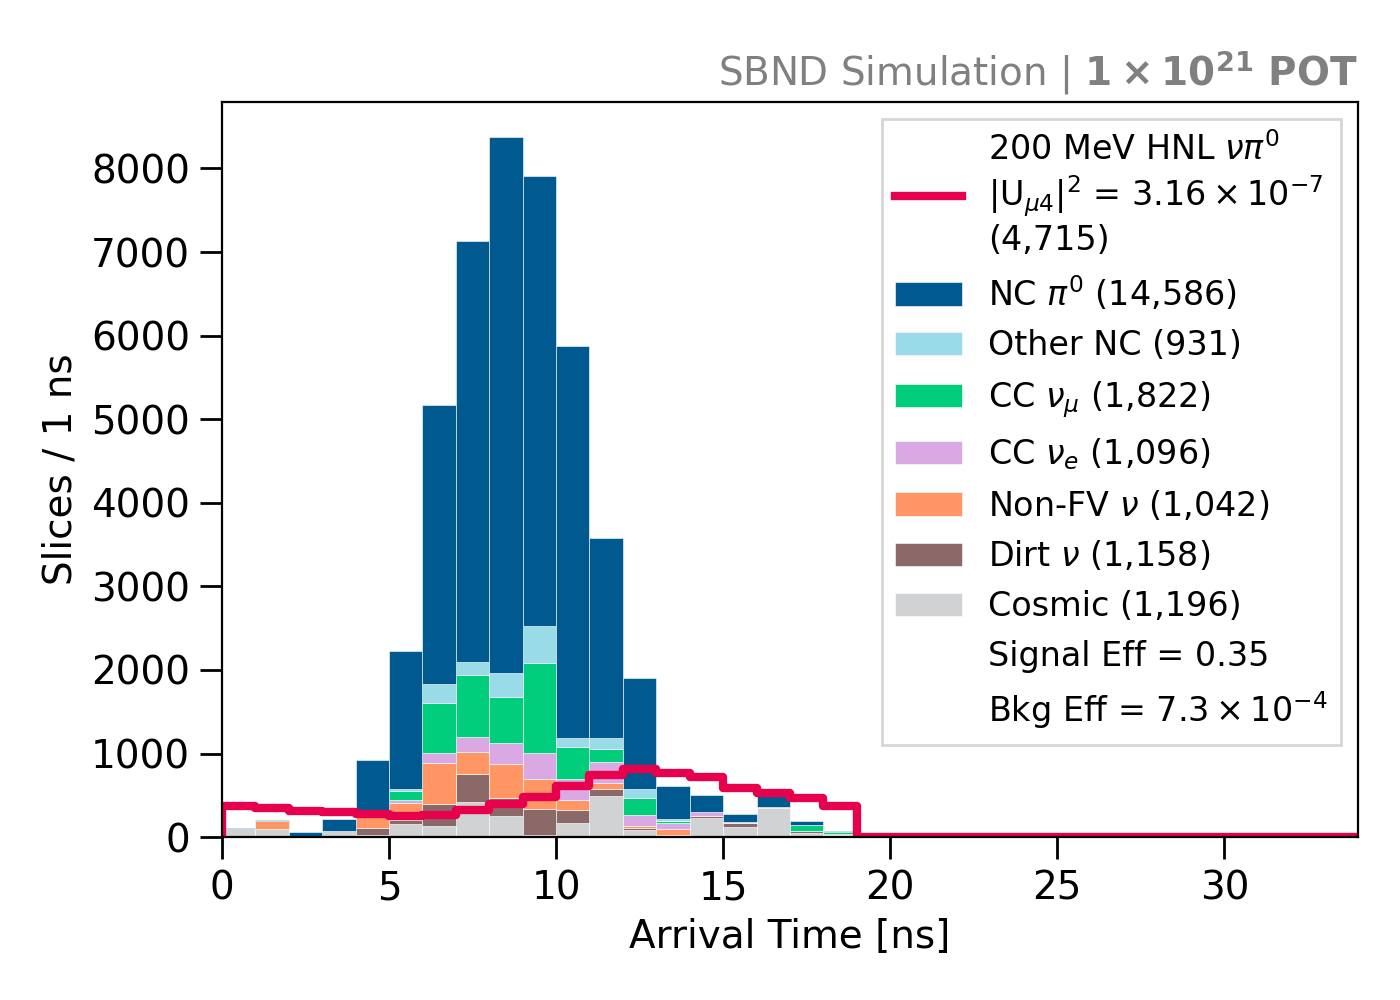
\includegraphics[width=\textwidth]{beam_bucket_postopt0}
            \caption{After Calorimetry cut}%
	    \label{fig:bb_opt0}
        \end{subfigure}
        \caption{
		Plots demonstrating the calorimetry cut (top) and the resulting beam bucket distribution after the cut (bottom). 
	}
        \label{fig:opt0_cut}
\end{figure}

The overestimation is demonstrated in Fig. \ref{fig:opt0_cut}, where HNL slices mainly concentrate in the region $\frac{(L_{\mathrm{Q}} - L)}{L} \geq 0$. 
The calorimetry cut exploits this feature and is tuned towards the single shower and multiple shower case.
For slices containing a single shower, the requirement on the fraction is between -0.1 and 0.4 to select well-predicted showers with the fraction centred around 0, as well as overestimated showers with the fraction $> 0$. 
For slices containing multiple showers, the requirement on the fraction is restricted to only between 0.04 and 0.3 to strictly select only overestimated showers, rejecting backgrounds more aggressively.
The beam bucket distribution after the cut is shown in Fig. \ref{fig:bb_opt0}, demonstrating the effectiveness of the cut as the background rejection efficiency increases by a whole order of magnitude from $\mathcal{O}(10^{-3})$ to $\mathcal{O}(10^{-4})$. 
Meanwhile, the signal selection efficiency only decreases from 43\% to 35\%.

\subsection{Theta Angle Cut}

The fourth cut of the HNL shower selection exploits the geometry of the forward-going HNL showers such that their theta angles with respect to the beam direction are small.                                      
Fig. \ref{fig:1shw_theta_cut} shows the distribution of theta angle for slices containing a single shower.                                                                                                   
In this case, the signal is mainly highly energetic and boosted di-photons showers reconstructed as a single merged and collimated shower.
Their theta angles mainly dominate in the low theta region.
A strict selection of $< 25^{\circ}$ can be placed without compromising signal efficiency due to the high signal-to-background ratio in this region.
Fig. \ref{fig:2shw_theta_cut} shows the theta angle distribution for slices containing multiple showers.
In this case, HNL showers are less boosted and more likely to result in separated showers.
Their theta angles with respect to the beam are larger compared to the single shower case.
To preserve signal selection efficiency, a widened selection of $< 30^{\circ}$ is applied.

Fig. \ref{fig:bb_theta} shows the beam bucket distribution after applying the cut.
The theta angle cut effectively rejects any shower-like backgrounds that are not collimated, resulting in a reduction across all SM neutrino interaction types.
This is a very impactful cut given that the background rejection efficiency increases by half from $7.3 \times 10^{-4}$ to $3.6 \times 10^{-4}$.
Meanwhile, the signal selection efficiency of HNL slices only drops by 2\%.

\begin{figure}[h!]
        \begin{subfigure}[b]{0.495\textwidth}   
            \centering 
            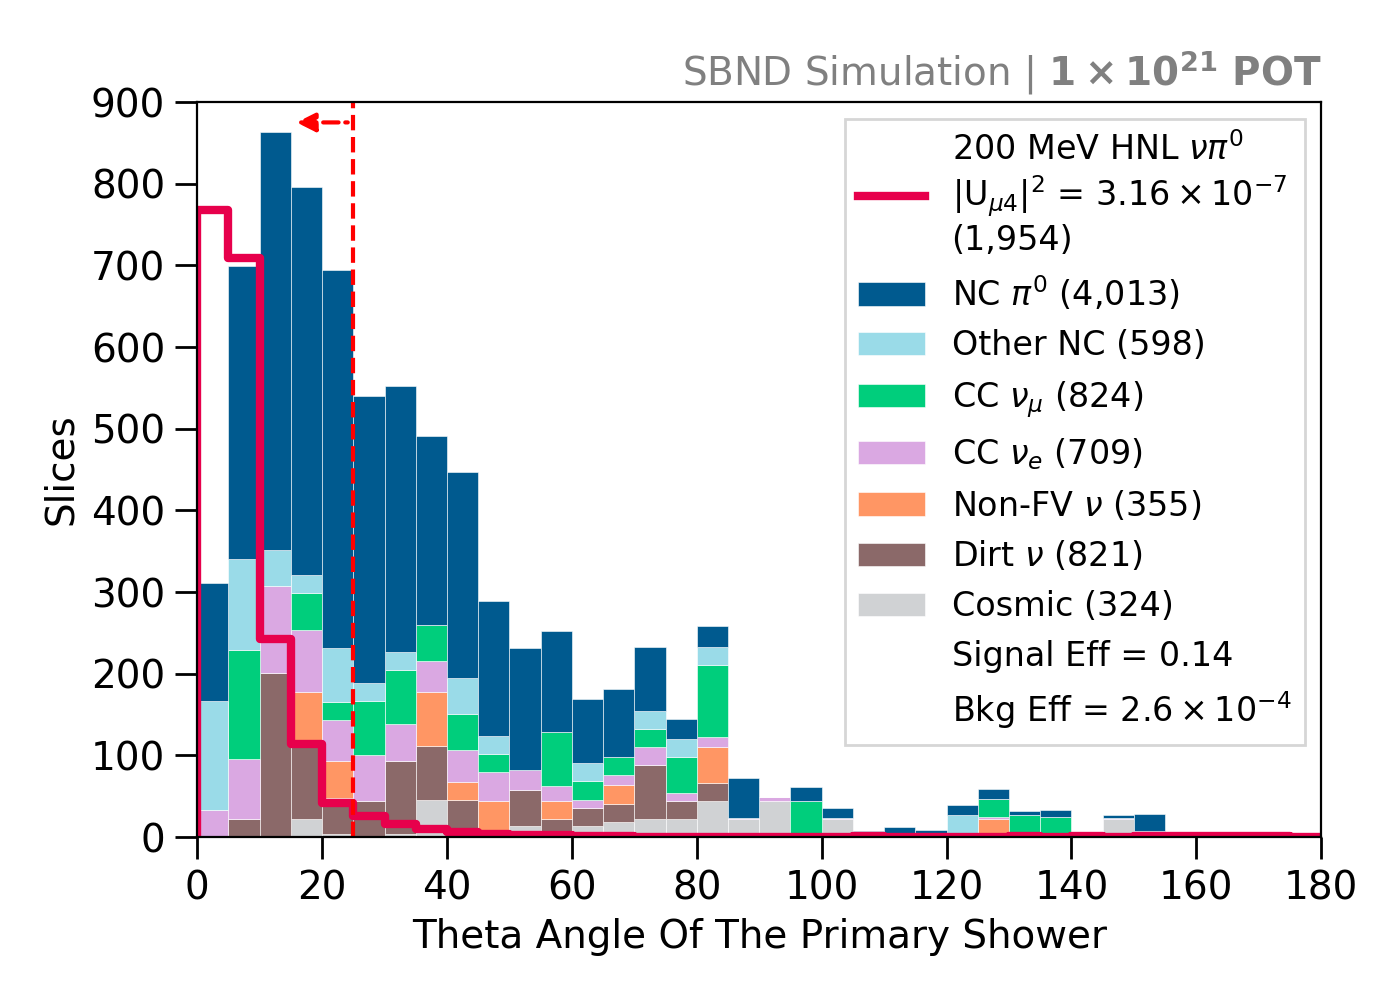
\includegraphics[width=\textwidth]{one_shower_theta_precut}
            \caption{1 Shower Case: Shower theta cut}%
	    \label{fig:1shw_theta_cut}
        \end{subfigure}
        \hfill
        \begin{subfigure}[b]{0.495\textwidth}   
            \centering 
            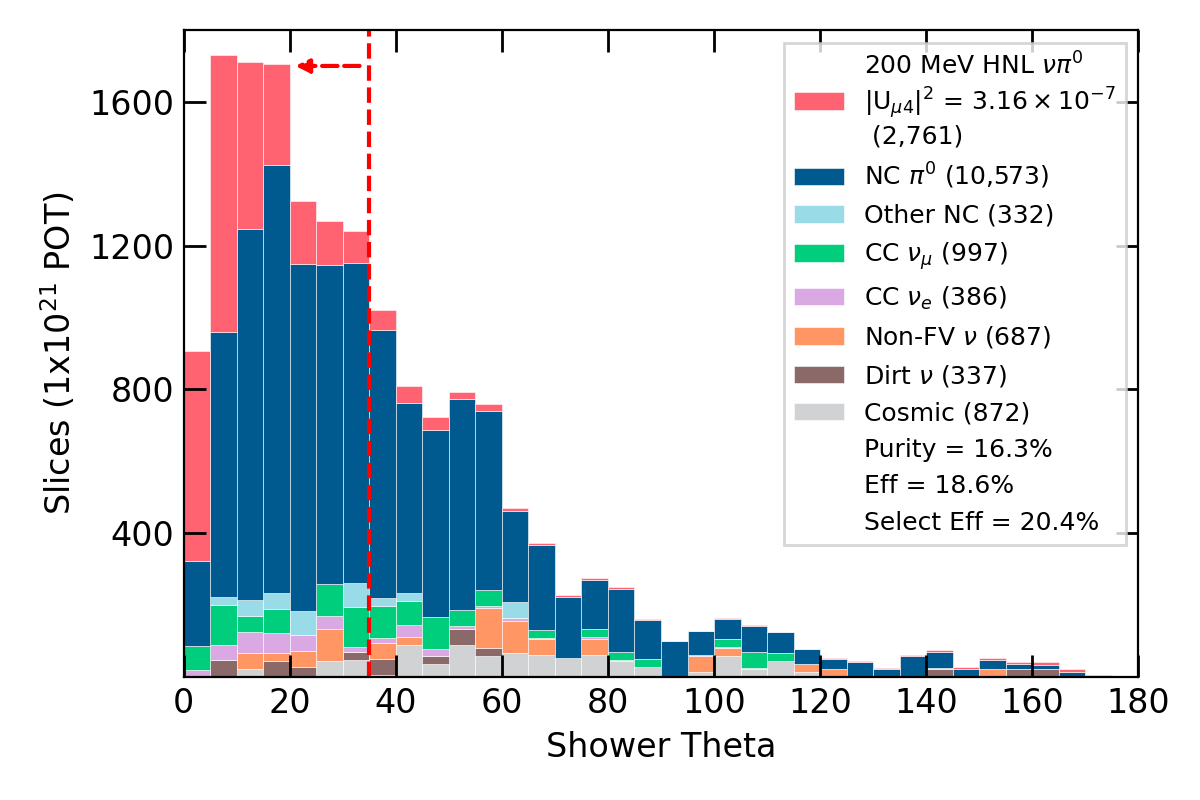
\includegraphics[width=\textwidth]{two_shower_primary_theta_precut}
            \caption{2+ Showers Case: Shower theta cut}%
	    \label{fig:2shw_theta_cut}
        \end{subfigure}
        \hfill
	\centering
        \begin{subfigure}[b]{0.495\textwidth}   
            \centering 
            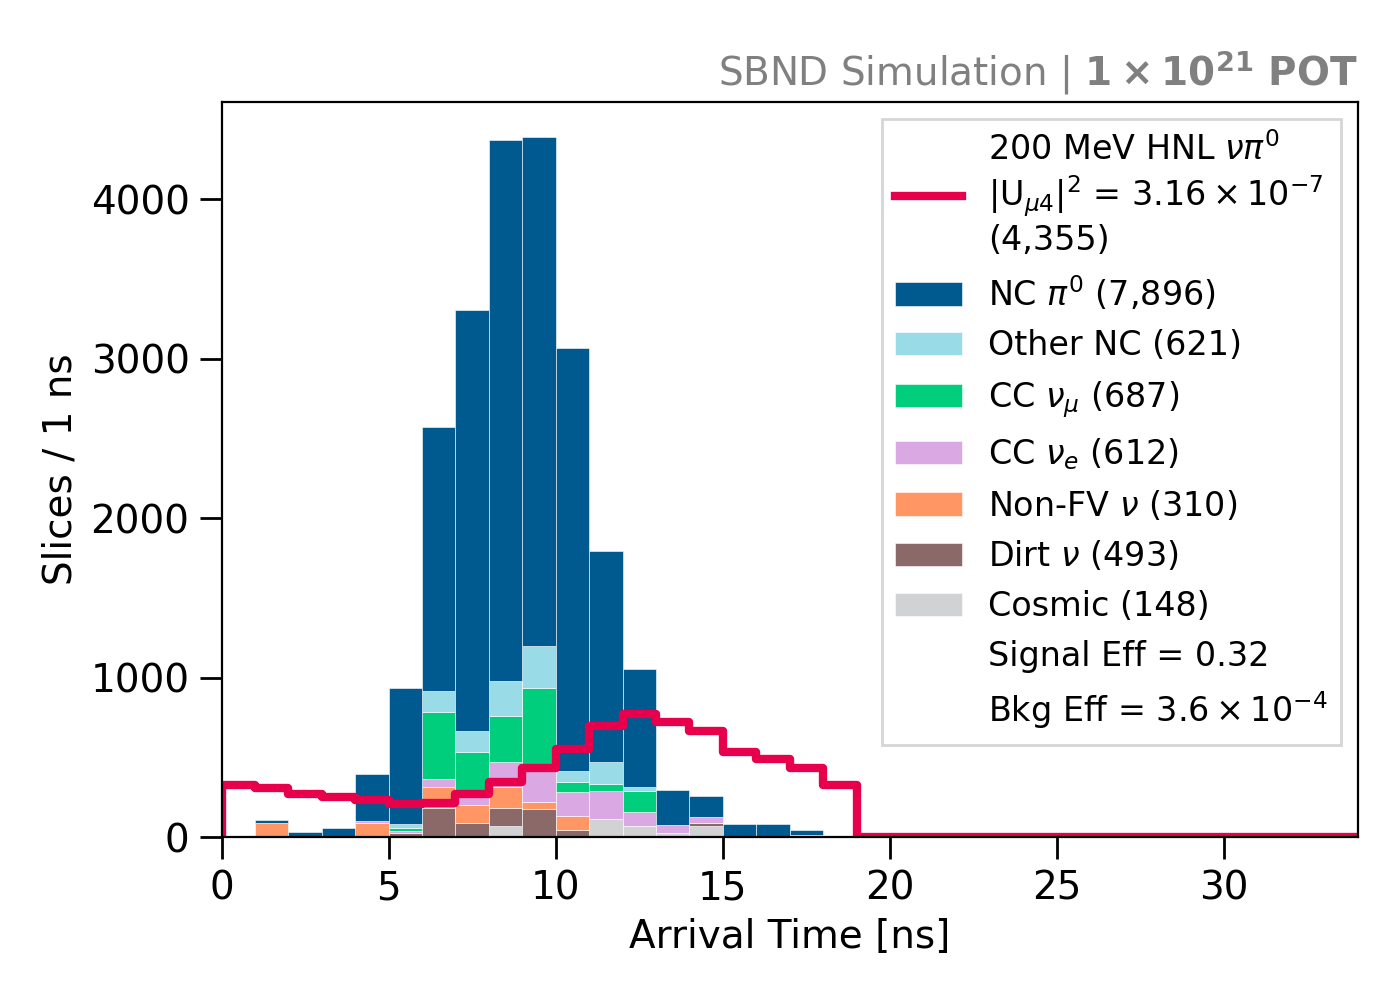
\includegraphics[width=\textwidth]{beam_bucket_postshowertheta}
            \caption{After shower theta cut}%
	    \label{fig:bb_theta}
        \end{subfigure}
        \caption{
		Plots demonstrating the shower theta cut (top) and the resulting beam bucket distribution after the cut (bottom). 
	}
        \label{fig:theta_cut}
\end{figure}

\subsection{Invariant Mass Cut}

The final cut of the HNL shower selection is to exploit the fact that di-photon showers originate from a $\pi^0$ decay, allowing for an invariant mass reconstruction.
For slices containing multiple showers, the invariant mass can be constructed using the reconstructed momenta of any 2 showers combination in the slice.
For 2 massless photon showers with an opening angle $\alpha$ and a total energy $E_1$ and $E_2$ respectively, the parent $\pi^0$ invariant mass is computed as follows
\begin{equation}
	m_{\pi^0} = \sqrt{2 E_1 E_2 \times (1 - \mbox{cos}\alpha)}
\end{equation}
For a given slice, the $\pi^0$ invariant mass is reconstructed for all combinations of 2 showers, and the closest mass is considered.
The cut is illustrated in Fig. \ref{fig:mass_cut}, where the solid red line indicates the $\pi^0$ mass of 135 MeV.
A cut is applied to select slices corresponding to a reconstructed invariant mass of 300 MeV or less.
This rejects any slices with a poorly reconstructed $\pi^0$ mass, which could be due to backgrounds from 
SM neutrino interactions such as CC $\nu_\mu$, other NC, Non-FV and dirt as well as energetic cosmic rays.
However, poor shower reconstruction can also result in di-photon showers from $\pi^0$ getting mistakenly rejected by this cut, as it is evident that some NC $\pi^0$ interactions and HNL signals are affected.
This cut minimally reduces both signal and background slices to less than $3 \%$.

\begin{figure}[h!]
        \centering 
        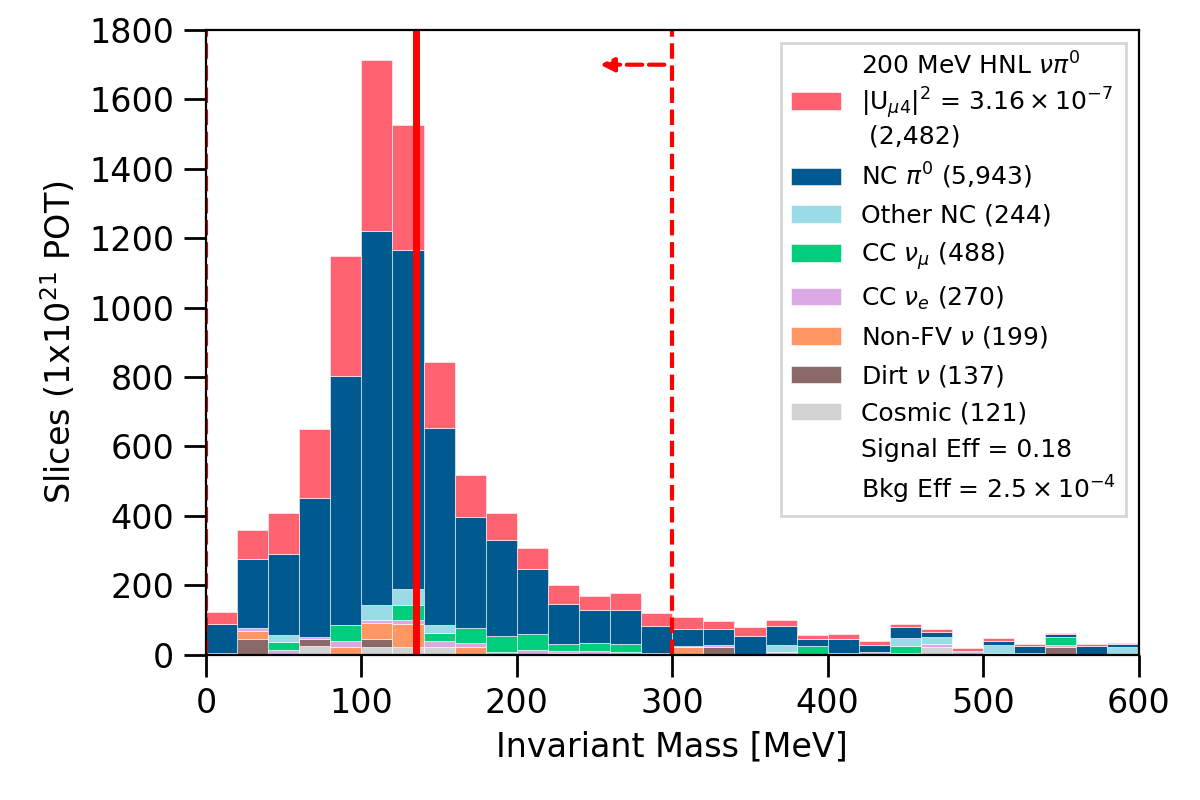
\includegraphics[width=0.495\textwidth]{pizero_mass_precut}
	\caption{
	Plots demonstrating the $\pi^0$ invariant mass cut applied to the multiple showers case.
	}
        \label{fig:mass_cut}
\end{figure}

\section{Final Selection Result}
\label{sec:select_result}

Fig. \ref{fig:bb_full_loose} shows the beam bucket distribution after the whole selection procedure.
The background efficiency shown in the plot is $3.3 \times 10^{-4}$, demonstrating the extreme background rejection required for this analysis by four orders of magnitude.
Meanwhile, the signal selection efficiency is still well-preserved as $30\%$ of the HNL slices remain. 
The peak region of the bucket is still dominated by the primary background from NC $\pi^0$ interactions which have proven to be a very tricky background to remove due to their similarity with HNL showers.
Moreover, a fraction of CC $\nu_e$ interactions persists as they can produce a single shower topology. 
A combination of CC $\nu_\mu$, other NC, Non-FV and dirt neutrino interactions remain even though they were not considered to be a background at the beginning.
These interactions likely undergo deep inelastic scattering, producing shower-like products like $\pi^0$ or $e^{\pm}$.

The multi-binned analysis for setting limits depends on the signal-to-background ratio per bin, of which signal-rich bins drive the limits.
Fig. \ref{fig:bb_edge_loose} zooms into the first and last 4 bins of the beam bucket distribution, which are the highest purity of the entire histogram.
These edge bins contribute towards the final sensitivity limits significantly more than other bins located at the peak region. 
Thus, a \textit{timing cut} might be applied to select only these bins, which would result in a background rejection efficiency increasing from $\mathcal{O}(10^{-4})$ to $\mathcal{O}(10^{-6})$ while still maintain 10\% of signal efficiency.
However, the cut is not formally applied as part of the selection procedure, but only to highlight the importance of these edge bins, particularly to demonstrate their excellent signal-to-background ratio.
The timing cut will be discussed in Chapter \ref{ChapterResult} when setting upper limits using the beam bucket distribution.

\begin{figure}[b!]
	\hfill
	\begin{subfigure}[b]{0.495\textwidth}   
            \centering 
            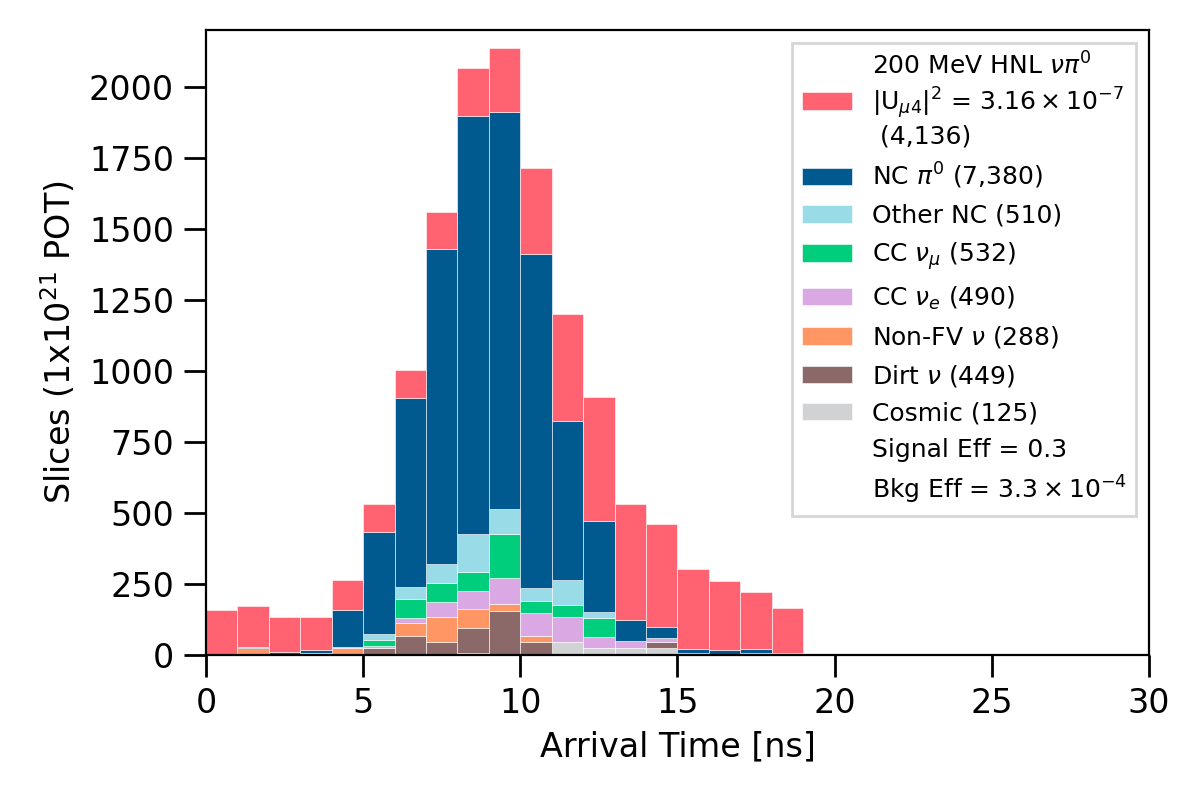
\includegraphics[width=\textwidth]{bb_lenient_full}
            \caption{Lenient Cut: Full beam bucket}%
	    \label{fig:bb_full_loose}
        \end{subfigure}
        \hfill
	\begin{subfigure}[b]{0.495\textwidth}   
            \centering 
            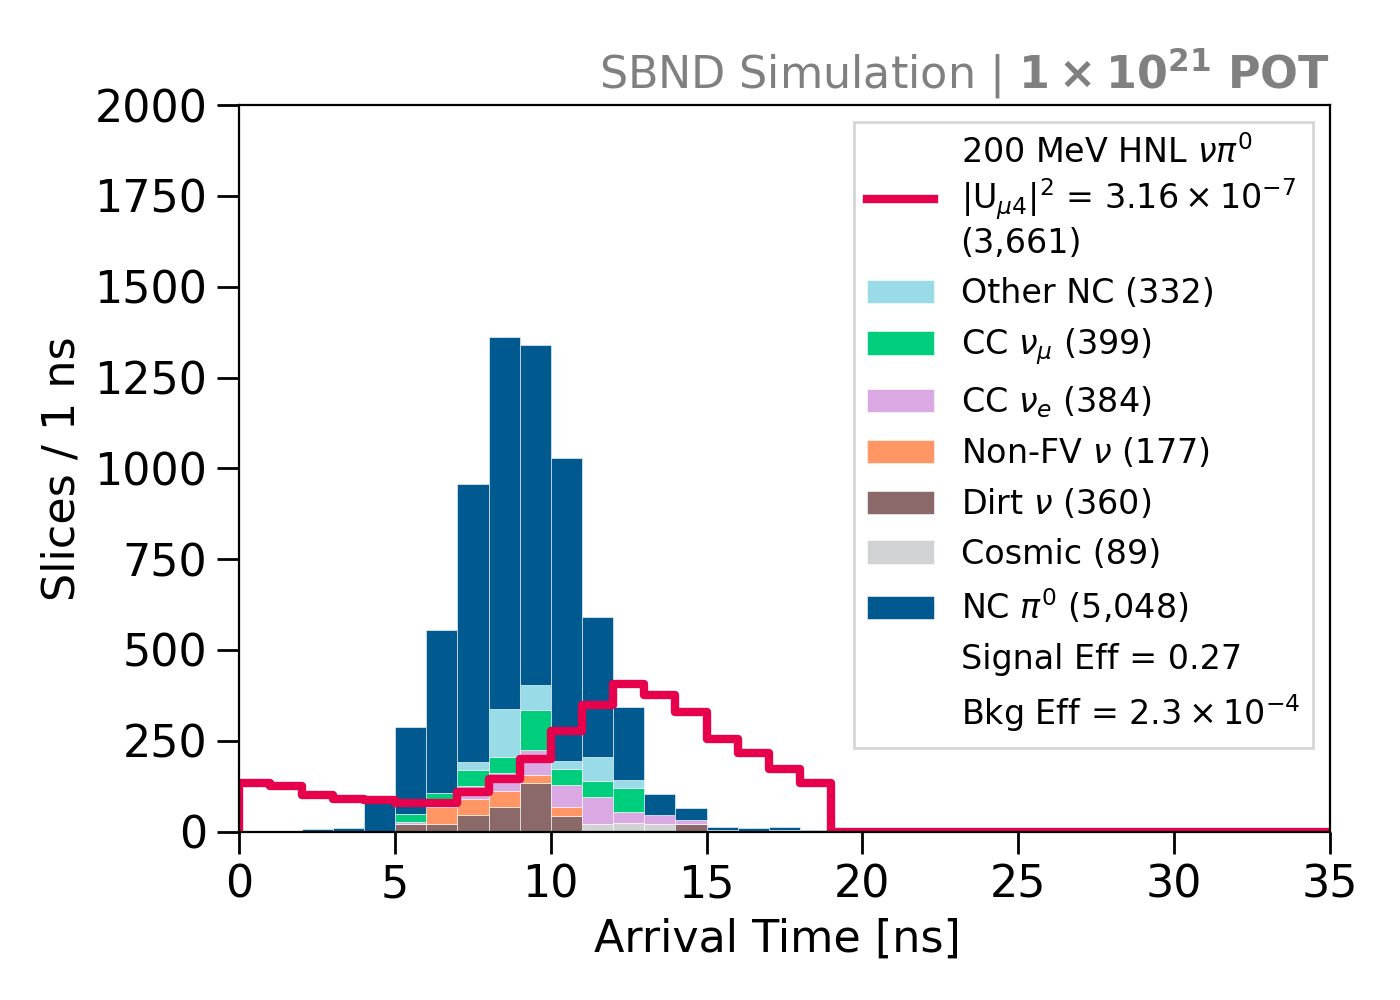
\includegraphics[width=\textwidth]{bb_stringent_full}
            \caption{Stringent Cut: Full beam bucket}%
	    \label{fig:bb_full_strict}
        \end{subfigure}
	\hfill
        \begin{subfigure}[b]{0.495\textwidth}   
            \centering 
	    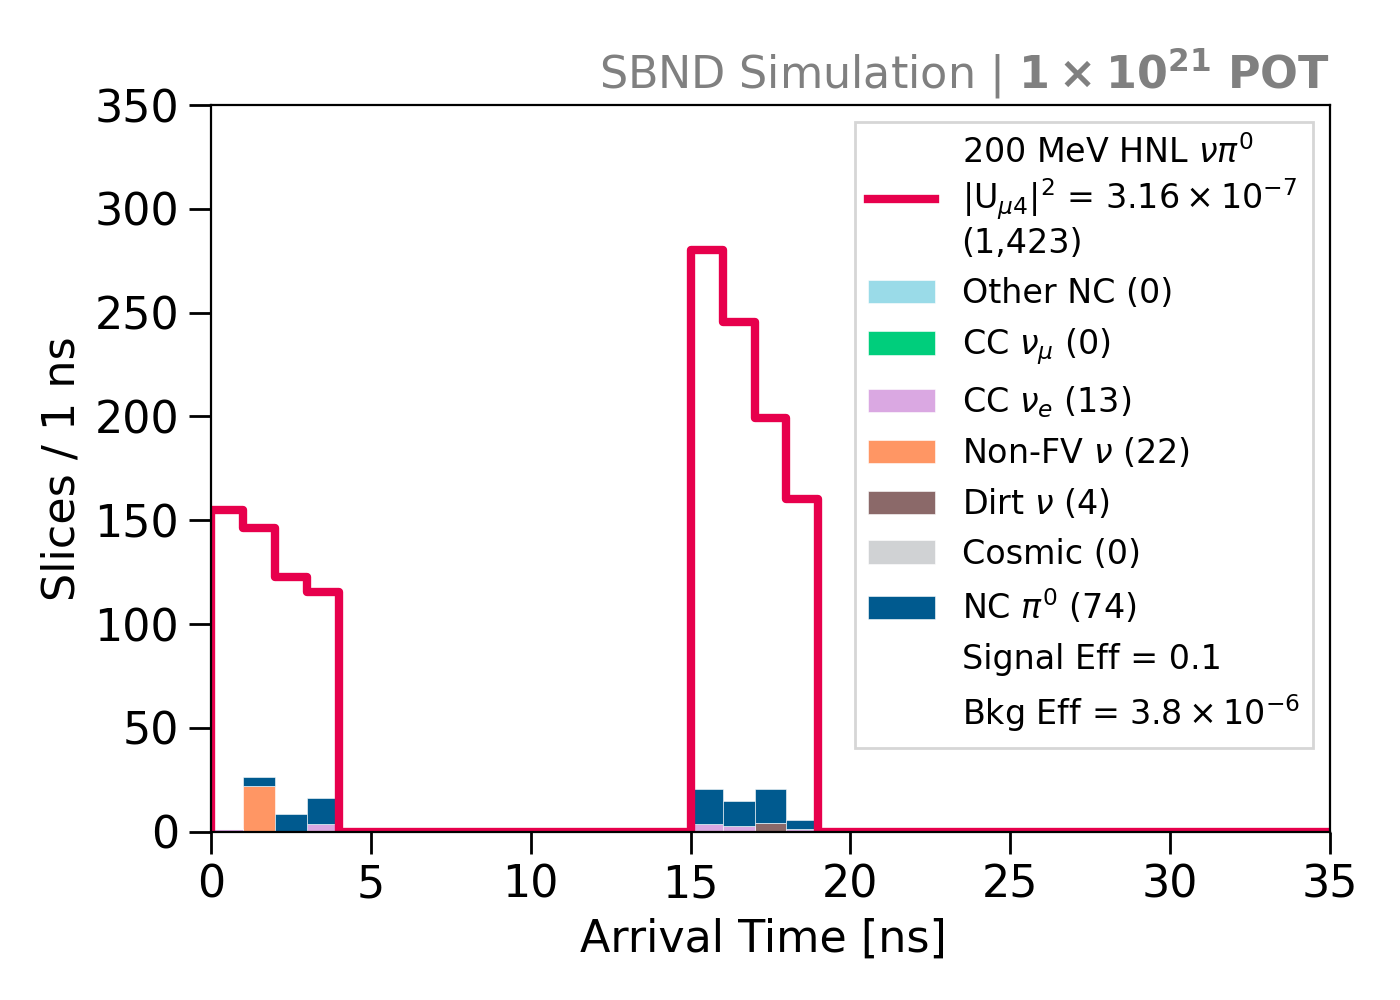
\includegraphics[width=\textwidth]{bb_lenient_edge}
            \caption{Lenient Cut: Edge of bucket}%
	    \label{fig:bb_edge_loose}
        \end{subfigure}
        \hfill
        \begin{subfigure}[b]{0.495\textwidth}   
            \centering 
	    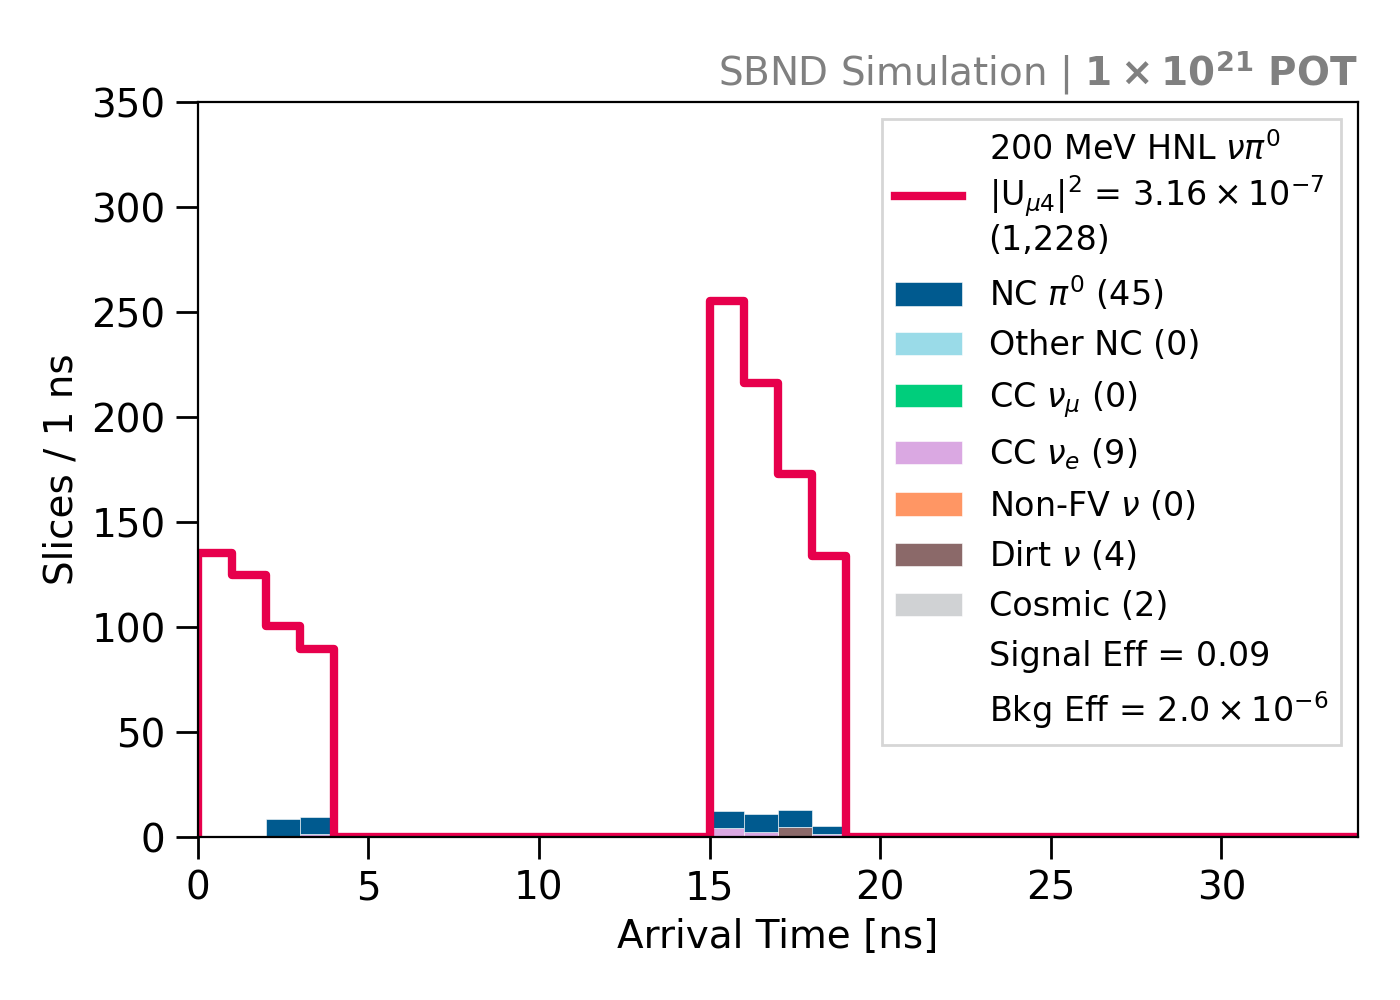
\includegraphics[width=\textwidth]{bb_stringent_edge}
            \caption{Stringent Cut: Edge of bucket}%
	    \label{fig:bb_edge_strict}
        \end{subfigure}
        \caption{
		Plots showing the final beam bucket distribution after selection.
	}
        \label{fig:timing_cut}
\end{figure}
To better understand the sensitivity limits dependency on the signal-to-background ratio, two selection procedures were developed.
The selection demonstrated up until this point is referred to as \textit{the lenient cut}.
An additional more aggressive cut, referred to as \textit{the stringent cut}, was developed by tightening the two most impactful cuts on calorimetry and theta angle. 
The resulting beam bucket distribution for the stringent cut is plotted in Fig. \ref{fig:bb_full_strict} 
and \ref{fig:bb_edge_strict} for the entire distribution and only the edge bins respectively. 
The key difference between these two cuts is that the lenient cut retains more signals however at a lower purity.
Meanwhile, the stringent cut results in higher purity at the cost of signal efficiency.
The two selections are summarised in Table \ref{table:cut_summary}.

Fig. \ref{fig:eff} shows the signal selection and background rejection efficiency cut by cut.
The signal selection efficiency is plotted using the left axis in pink and the background rejection efficiency is plotted using the right axis in blue.
It is important to note that the right axis is in the logarithm scale as the background rejection is very aggressive.
The band of signal selection efficiency corresponds to the efficiency across the entire mass range of HNLs from 140 to 260 MeV, with efficiency increasing with mass. 
The selection differs from the calorimetry cut onwards, where the lenient cut is shown in pink and the stringent cut is shown in red.
Overall, the most highlighted cuts are the muon/proton/pion cut for track removal, followed by the calorimetry and theta angle cut by exploiting the boosted topology of HNLs that significantly reject backgrounds without compromising signal efficiency.

\begin{figure}[ht!]
    \centering 
    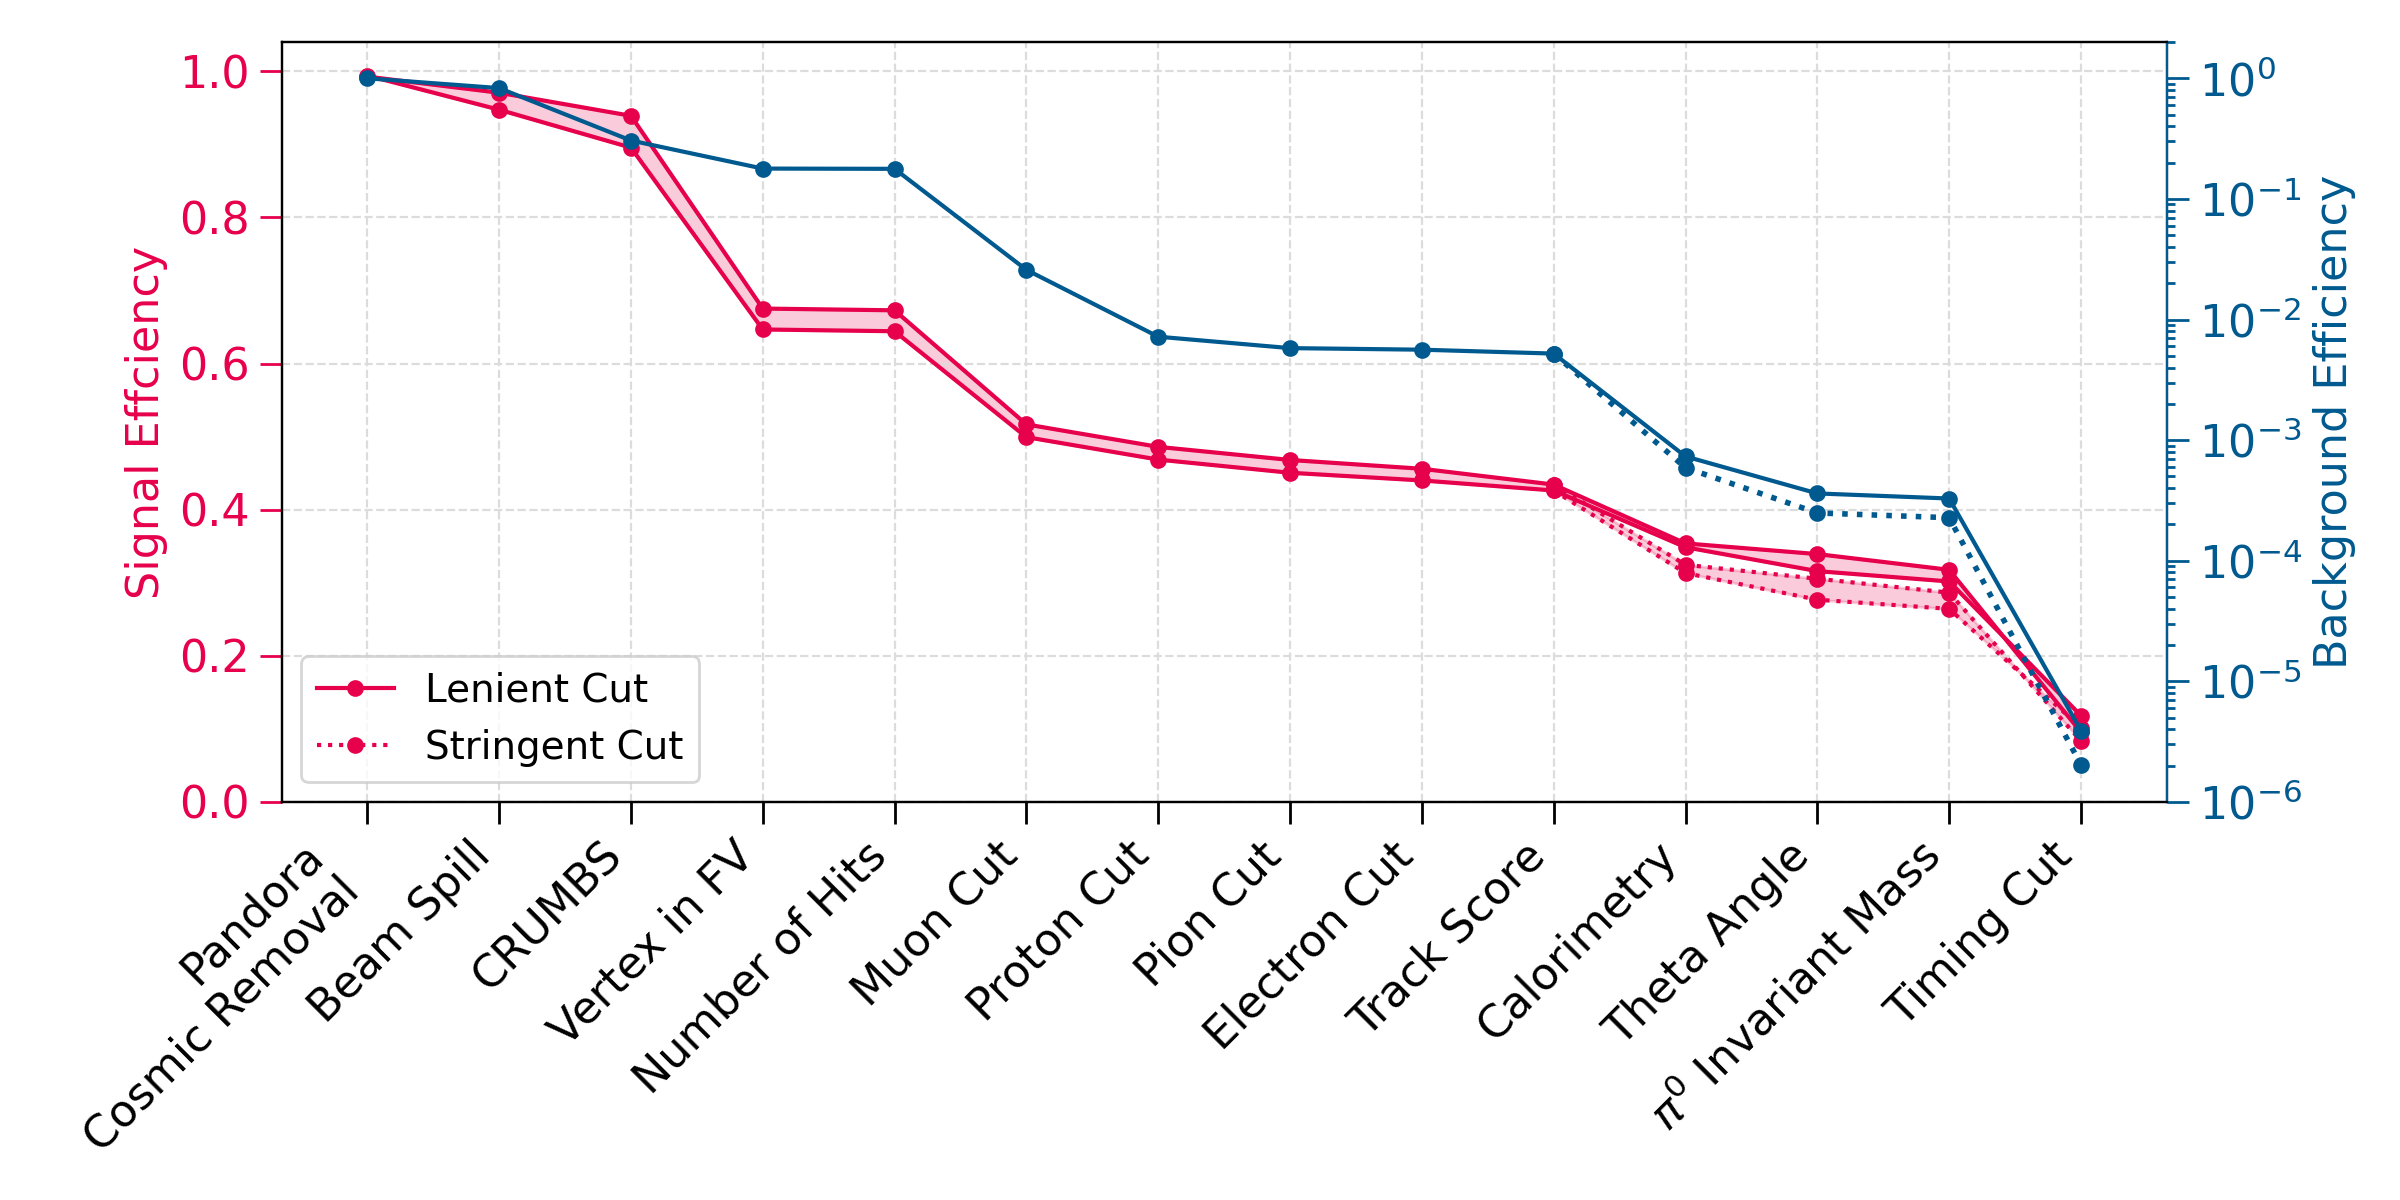
\includegraphics[width=1.0\textwidth]{peff_band}
    \caption{
		Plot demonstrating the signal selection efficiency (left axis) and the background rejection efficiency (right axis).
	}
        \label{fig:eff}
\end{figure}

\begin{table}[htbp!]
\centering
\begin{center}
\begin{tabular}{| p{7.75cm} | m{3.25cm} | m{3.25cm} |} 
 \hline
  & \multicolumn{2}{c|}{\textbf{Common Cut}} \\ [1ex] 
 \hline
 \textbf{Cosmic Removal}: & \multicolumn{2}{c|}{} \\ [1ex] 
 Slice reconstructed by Pandora as a neutrino & \multicolumn{2}{c|}{True} \\ 
 Flash time inside the beam spill & \multicolumn{2}{c|}{[0.367, 1.967] $\mu$s} \\ 
 CRUMBS score  & \multicolumn{2}{c|}{$\geq 0$} \\ [1ex] 
 \hline
 \textbf{SM Neutrino Removal}: & \multicolumn{2}{c|}{} \\ [1ex] 
 Reconstructed vertex inside the FV & \multicolumn{2}{c|}{True} \\
 \# of hits in the primary shower & \multicolumn{2}{c|}{$\geq 50$} \\ [1ex]
 \# of Razzled muons & \multicolumn{2}{c|}{0} \\
 Razzled muon score of particles in a slice & \multicolumn{2}{c|}{$< 0.04$} \\ [1ex]
 \# of Razzled protons with KE $>$ 32.7 MeV & \multicolumn{2}{c|}{0} \\
 Razzled proton score of particles in a slice & \multicolumn{2}{c|}{$< 0.96$} \\ [1ex]
 \# of Razzled pions with KE $>$ 31.2 MeV & \multicolumn{2}{c|}{0} \\
 Razzled pion score of particles in a slice & \multicolumn{2}{c|}{$< 0.82$} \\ [1ex]
 \hline
 \textbf{HNL Shower Selection}: & \multicolumn{2}{c|}{} \\ [1ex] 
 Razzled electron score of the primary shower & \multicolumn{2}{c|}{$< 0.96$} \\ [1ex]
 Track score of the primary shower & \multicolumn{2}{c|}{} \\
 \hspace{0.5cm}1 shower case & \multicolumn{2}{c|}{$0.225 <$ score $< 0.5$} \\
 \hspace{0.5cm}2+ shower case & \multicolumn{2}{c|}{$0.250 <$ score $< 0.5$} \\
 \cline{2-3}
 & \multicolumn{1}{c|}{\textbf{Lenient Cut}}  & \multicolumn{1}{c|}{\textbf{Stringent Cut}} \\  
 \cline{2-3}
 (L$_\mathrm{Q}$ - L) / L fraction of a slice &  &  \\
  \hspace{0.5cm} 1 shower case & \multicolumn{1}{c|}{$-0.12 <$ frac $< 0.40$} & \multicolumn{1}{c|}{$-0.10 <$ frac $< 0.40$} \\
  \hspace{0.5cm} 2+ showers case & \multicolumn{1}{c|}{$\ \ \ 0.00 <$ frac $< 0.40$} & \multicolumn{1}{c|}{$\ \ \ 0.04 <$ frac $< 0.30$} \\ [1ex]
  Theta angle of the primary shower &  &  \\
  \hspace{0.5cm}1 shower case & \multicolumn{1}{c|}{$\leq 25^\circ$} & \multicolumn{1}{c|}{$\leq20^\circ$} \\
  \hspace{0.5cm}2+ showers case & \multicolumn{1}{c|}{$\leq 35^\circ$} & \multicolumn{1}{c|}{$\leq 30^\circ$} \\ [1ex]
  \cline{2-3} 
  Invariant mass of any 2 showers in a slice  & \multicolumn{2}{c|}{$\leq 300$ MeV} \\ [1ex]
 \hline
 \textbf{Timing Cut *(applied when setting limits)}: &  \multicolumn{2}{c|}{} \\ [1ex] 
 Arrival time within the beam bucket  & \multicolumn{2}{c|}{$0 \leq t \leq 4$ and $15 \leq t \leq 19$} \\ [1ex]
 \hline
\end{tabular}
\end{center}
\caption{Table summarising the lenient and stringent selection.}
\label{table:cut_summary}
\end{table}


%********************************** %First Section  **************************************
\section{Truth Study On Timing Resolution Improvement}
\label{sec:truth_bucket}

In addition to the selection of reconstructed variables, a truth study was carried out to better the limitations of the reconstruction, particularly the timing resolution.
The truth study was performed on \textit{true} variables, indicating that no detector simulation and reconstruction were applied.

There are several factors smearing the arrival time of a SM neutrino at SBND, and consequently smearing the Gaussian shape of the beam bucket, as depicted in Fig. \ref{fig:smearing_factors}.
The intrinsic Gaussian sigma of the proton bucket from the Booster synchrotron is 1.308 ns, as shown by the brown arrow.
This structure is then smeared out due to the Time of Flight (ToF) of secondary mesons, as shown by the purple arrow.
Moreover, the ToF of the tertiary particles, whether SM neutrinos or HNLs, from the production location to the detector further smears the Gaussian, as shown by the pink arrow.
Once the particle arrives at the detector, two additional smearing factors need to be considered.
The first one is the particle ToF inside the detector, as shown by the red arrow.
The second one is the ToF of the photon from the production to the detection location, assuming the production location is close to the interaction vertex, as shown by the green arrow.

\begin{figure}[h!]
    \centering
    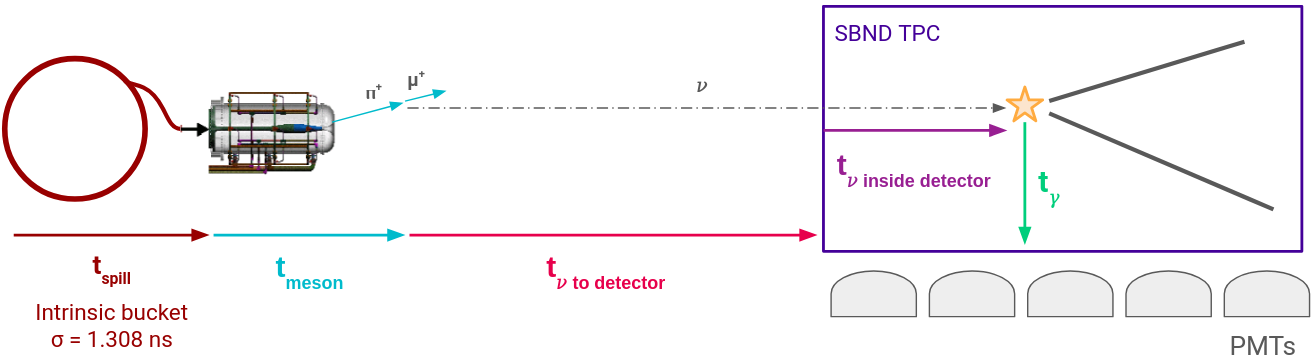
\includegraphics[width=1.0\textwidth]{smearing_factors.png}
    \caption{Diagram showing different smearing contributors to the beam bucket distribution.}
    \label{fig:smearing_factors}
\end{figure}

The truth beam bucket of SM neutrinos that arrive at the front face of SBND is plotted in the left figure of Fig. \ref{fig:gaus_truth_reco}.
This distribution was computed using the true interaction time at the vertex, marked by the yellow star in Fig. \ref{fig:smearing_factors}, and then corrected for the SM neutrino ToF inside the detector, depicted by the red arrow.
In the truth phase space, it is evident that the combination of the ToF of the secondary mesons and of SM neutrinos to the detector smears the Gaussian sigma by a negligible amount from 1.308 ns to 1.37 ns.

The reconstructed beam bucket distribution of SM neutrinos is plotted in the right figure of Fig. \ref{fig:gaus_truth_reco}.
As previously detailed in Sec. \ref{sec:key_dist}, the beam bucket is reconstructed using the flash time matched a slice.
The flash time, as detailed in Sec. \ref{sec:reco_pds}, was reconstructed using the prompt light occurring in the first 30 ns of the flash window such that the scintillation location is close to the interaction vertex.
Moreover, the flash time was already corrected for the photon propagation time drifting from the scintillation location to PMTs, depicted by the green arrow in Fig. \ref{fig:smearing_factors}.
Then, the SM neutrino ToF inside the detector, as shown by the red arrow, was corrected by applying a shift from the reconstructed vertex $z$-position to $z = 0$ at the detector's front face.
Thus, the reconstruction depends on 3 variables: (1) the matching of flash-to-slice, (2) the flash time and (3) the slice vertex.
Each of these variables has its own reconstruction resolution and can smear the Gaussian shape of SM neutrinos arriving at the detector.
%The resulting beam bucket corresponds to a Gaussian with a sigma smeared from 1.308 ns to 2.26 ns.

%The right figure was made using the Rockbox sample, selecting only slices that match a true neutrino. 
%No cosmic slices are considered for simplification, however, having cosmics background can additionally smear the structure.
%Both truth and reco plots are normalised for direct comparison.

Going from the truth phase space to the reconstruction phase space, two observations can be made.
The first one is the shift of the Gaussian mean from 7.44 to 9.26, equivalent to a shift of 1.82 ns.
A portion of the shift is due to the reconstructed flash time introducing a shift of 1.45 ns \cite{sbnd_pds_paper}.
The remaining shift amount might be due to the slice vertex reconstruction and the flash matching.      
The second observation is that the Gaussian sigma is smeared from 1.37 ns to 2.26 ns. 
This sigma smearing is detrimental to the HNL search since it results in more SM neutrinos at the edge of the beam bucket and thus, reducing the signal-to-background ratio in this region.                     

\begin{figure}[htbp!]
    \vspace{1cm}
    \centering
    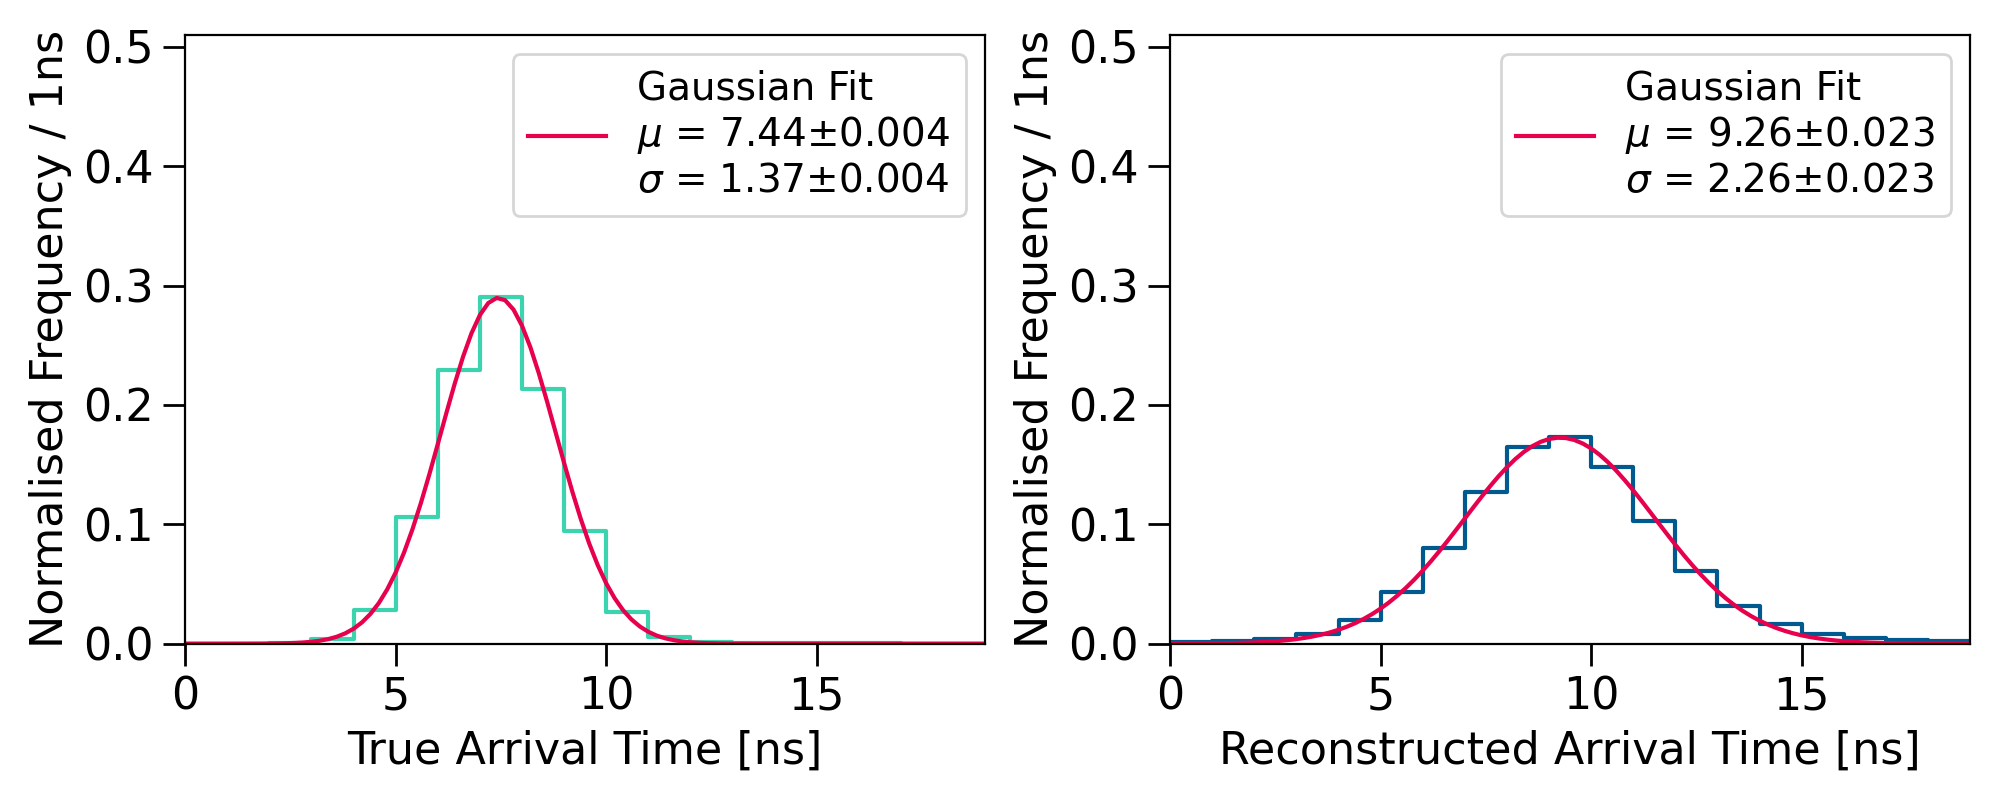
\includegraphics[width=0.75\textwidth]{truth_reco_gaus.png}
    \caption{Plots showing the beam bucket distribution of SM neutrinos in the truth phase space (left) and in the reconstruction phase space (right).}
    \label{fig:gaus_truth_reco}
\end{figure}

A hypothetical question is then proposed, ``How much can the sensitivity limits be improved if better timing resolution is achieved?''
This is equivalent to reconstructing the beam bucket distribution with less smearing under the two assumptions as follows
\begin{enumerate}
    \item A shifted Gaussian mean of 1.45 ns
    \item A smeared Gaussian sigma of 1.73 ns
\end{enumerate}
The Gaussian mean shift of 1.45 ns is motivated by the number reported by Ref. \cite{sbnd_pds_paper} detailing the light reconstruction in SBND. 
The Gaussian smeared sigma of 1.73 ns was motivated by the MicroBooNE experiment reporting on their intrinsic timing resolution \cite{uboone_ns}.
Although ambitious, it is an achievable goal for SBND to have a reconstructed timing resolution $< 2$ ns, given that SBND employs a very similar detector technology to MircoBooNE.
Moreover, Chapter \ref{ChapterDAQ} details the excellent timing performance of the DAQ system at SBND and the hardware preparation that already took place to achieve better timing resolution.
Particularly, the SPEC-TDC device, as previously discussed in Sec. \ref{subsec42TimeRef}, provides additional recorded timing information on the trigger and beam arrival that can only improve downstream reconstruction once incorporated. 

For modelling the background with these assumptions, only SM neutrinos are considered and not cosmics for simplification. 
The truth beam bucket distribution of SM neutrinos is first smeared with the two assumptions.
Then, to compare the new \textit{smeared truth} distribution to the reconstructed distribution \textit{after selection}, the smeared truth distribution is normalised to same area.
%For example, the lenient selection leaves 9,761 background slices in the final distribution. 
%distributions normalised to the same area of the reconstructed distribution after selection. 
Fig. \ref{fig:gaus_truth_smear} shows the comparison of the truth, smeared truth and the reconstructed distribution after selection.
The left figure shows the truth distribution without any smearing applied with a sigma of 1.37 ns.
The middle figure shows the smeared truth distribution using the stated assumptions with a sigma of 1.73 ns.
The right figure shows the reconstructed distribution after applying the lenient selection with a sigma of 1.99 ns.
It is important to note the difference between the reconstructed beam bucket before and after selection such that the distribution after selection has a less shifted Gaussian mean and a smaller Gaussian sigma.
This is due to cuts having non-uniform effects on the distribution. 

\begin{figure}[ht!]
    \centering
    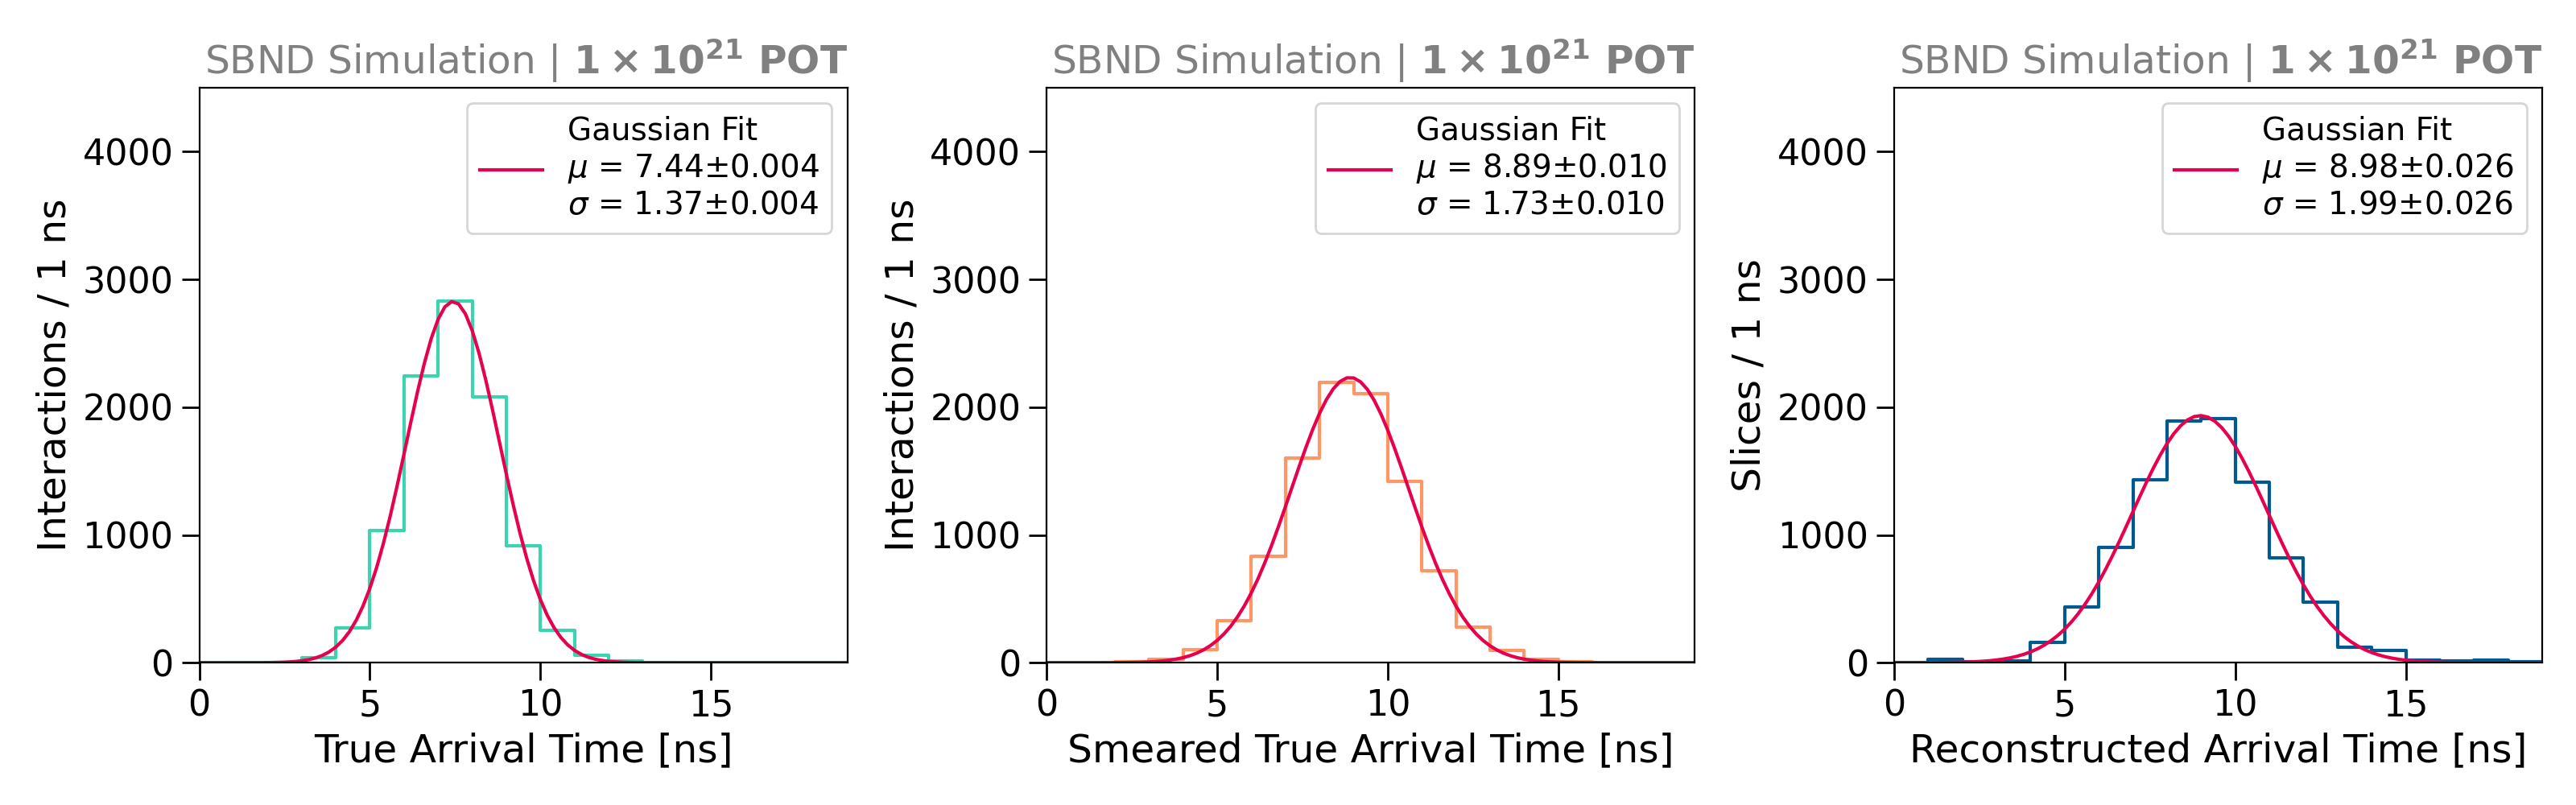
\includegraphics[width=\textwidth]{truth_smear_reco_gaus.png}
    \caption{Plots showing the beam bucket distribution of SM neutrinos in truth (left), smeared truth (middle) and reconstruction after selection (right).}
    \label{fig:gaus_truth_smear}
\end{figure}

For modelling the signal, the same smearing assumptions are applied to the truth timing distribution of HNLs. 
%Unlike the background modelling approach of normalising the number of remaining background slices after selection, a flat efficiency of 30\% is applied to the HNL truth distribution to account for the effects of reconstruction and selection combined.
Unlike the background modelling approach of normalising the same area, a flat efficiency of 30\% is applied to the HNL truth distribution to account for the effects of reconstruction and selection combined.
Fig. \ref{fig:hnl_sm_smear} shows the beam bucket distribution of SM neutrinos and HNLs across the phase space of truth, smeared truth and reconstruction after selection for comparison. 
The smeared truth distribution shows a higher signal-to-background ratio particularly for the bins at the edge of the bucket compared to the reconstructed distribution.
This smeared truth distribution will also used for setting the sensitivity limits alongside the reconstructed distributions, as this is an attempt to answer the proposed question on timing resolution improvement.

\begin{figure}[ht!]
    \centering
    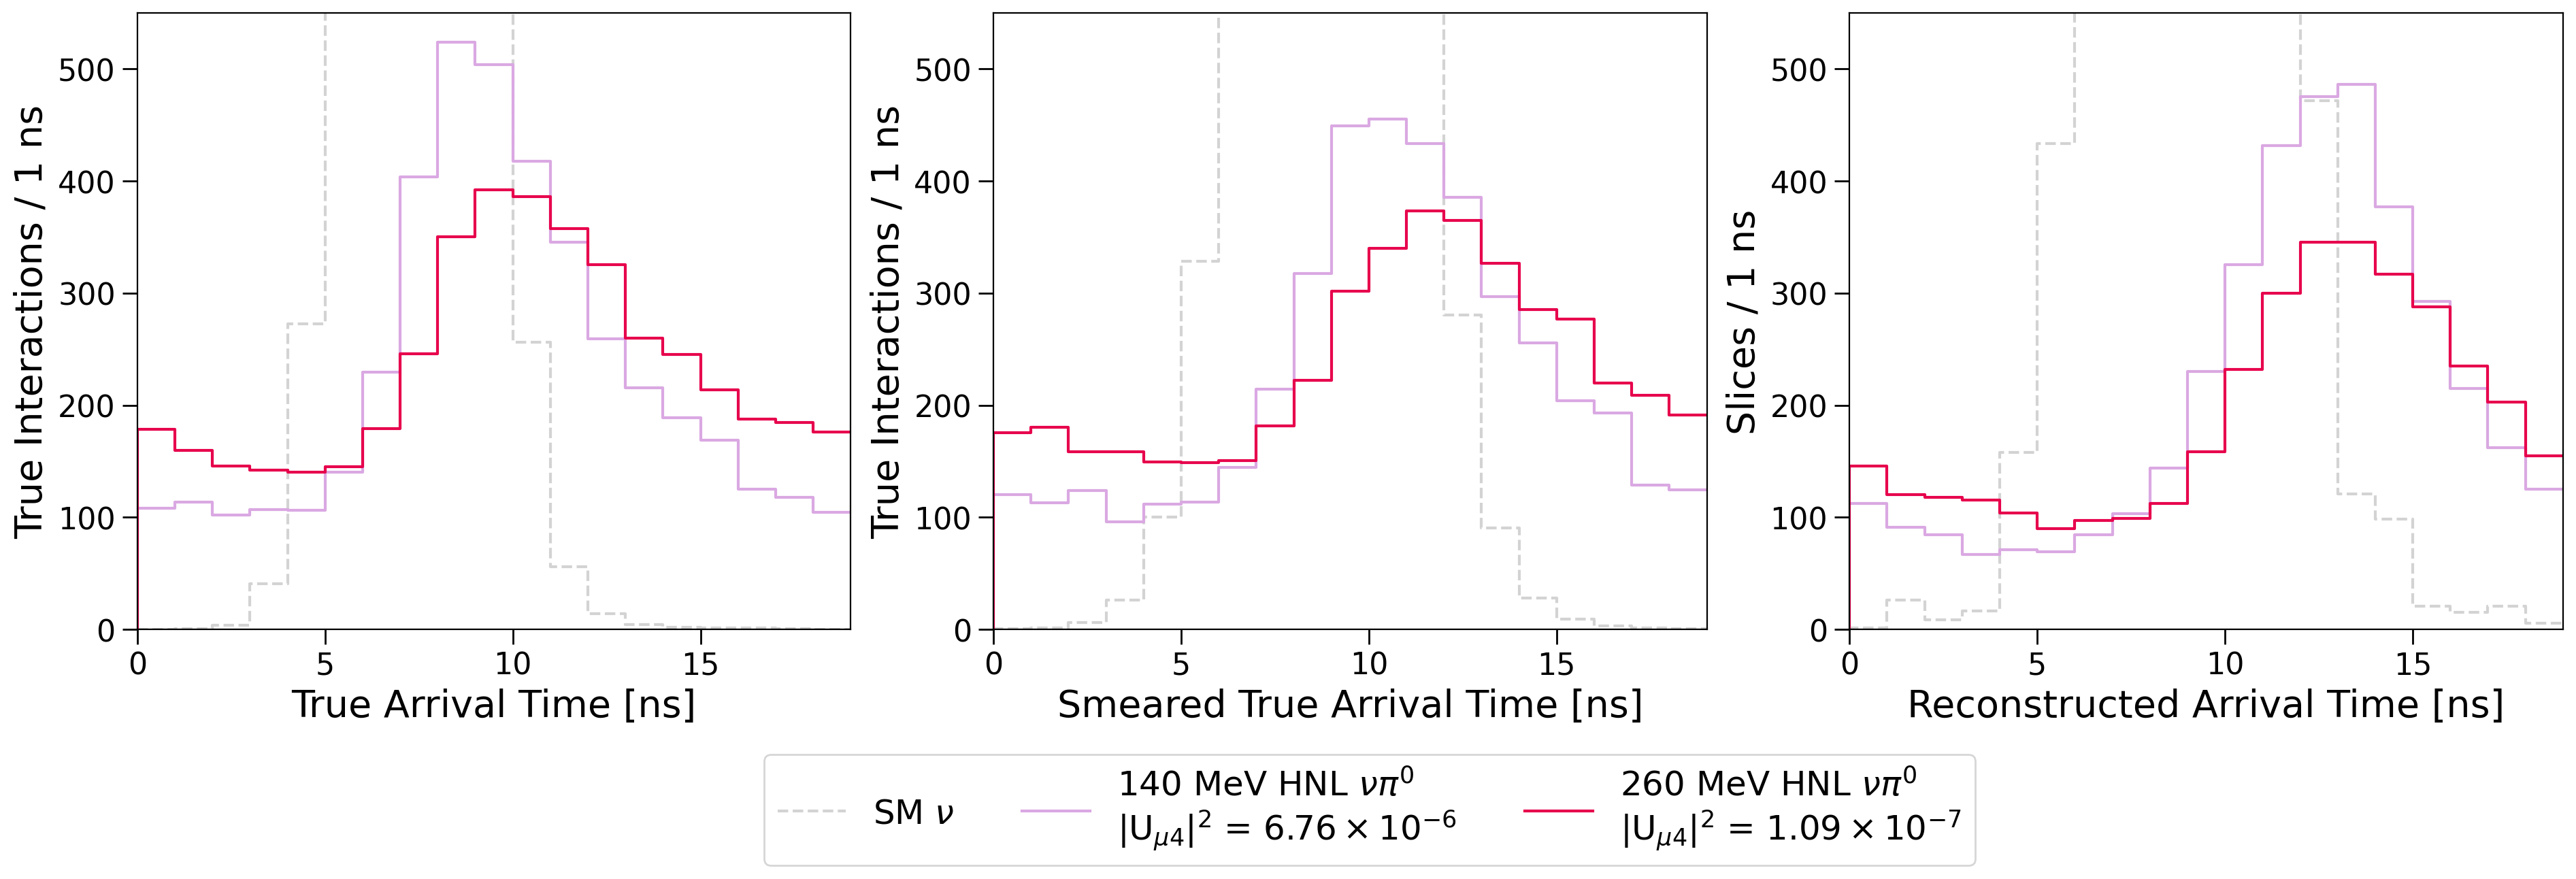
\includegraphics[width=\textwidth]{truth_smear_zoom.png}
    \caption{Plots showing the beam bucket distribution of SM neutrinos and HNLs in truth (left), smeared truth (middle) and reconstruction after selection (right).}
    \label{fig:hnl_sm_smear}
\end{figure}

%********************************** %First Section  **************************************

\section{Concluding Remarks}
\label{sec:select_conclude}

Both selection procedures presented here, the lenient and stringent cut, exploit the unique highly energetic and forward-going features of HNL showers to achieve an excellent background rejection efficiency without compromising signal selection efficiency.
The resulting background rejection efficiency is in the order of $\mathcal{O}(10^{-4})$ while the signal selection efficiency still maintains at 30\%. 
When considering only bins at the edge of the beam bucket distribution, or the so-called \textit{timing cut}, the background efficiency increases by two orders of magnitude to $\mathcal{O}(10^{-6})$ while the signal efficiency only reduces to 10\%. 
This is evident that these edge bins contain an exceptional signal-to-background ratio, which is the main factor driving the sensitivity limits.
Furthermore, a hypothetical question was proposed to explore the impact on sensitivity limits if the timing resolution is improved when reconstructing the beam bucket distribution.
All three beam bucket distributions, from both the lenient and stringent cut on reconstructed variables and from the smeared truth variables, will be used for setting upper limits on the mixing angle $|U_{\mu4}|^2$ of HNLs in the forth coming Chapter \ref{ChapterResult}. 


%Thus, the signal-to-noise ratio varies bin-by-bin, where signal-rich bins locate at the edge of the beam bucket (or the Gaussian tails) and background-rich bins locate at the centre of the beam bucket (or the Gaussian peak).
%The setting limits procedure, to be detailed in upcoming Chapter \ref{ChapterResult}, employs a multi-binned analysis such that the resulting sensitivity limits depends on the signal-to-noise ratio per bin.
%This implies that signal-rich bins are the main factor driving the limits.
%With this in mind, the following selection procedure was optimised to achieve a high signal-to-noise ratio with bins located at the edge of the beam bucket distribution.
